\section{Refrigeration Equipment }\label{refrigeration-equipment}

\subsection{Overview}\label{overview-023}

EnergyPlus can model refrigerated case equipment consisting of a compressor rack, multiple refrigerated cases and walk-in coolers, secondary loop equipment, and~ optional heat reclaim air and water heating coils. The refrigerated case equipment models perform four major functions:

\begin{itemize}
  \item calculate the electric consumption of refrigerated cases and walk-in coolers connected to a compressor rack
  \item determine the impact of refrigerated cases and walk-in coolers on zone cooling and dehumidification loads (i.e., case credits), including the effects of HVAC duct configuration
  \item calculate the electric consumption and COP of the compressor rack, and the electric and water (if applicable) consumption related to cooling the compressor rack's condenser.
  \item determine the total amount of heat rejected by the compressor rack's condenser and store this information for use by waste heat recovery models (e.g., using Desuperheater heating coil (object: Coil:Heating:Desuperheater) as an air reheat coil for high humidity control in a supermarket)
\end{itemize}

The case and walk-in models account for nearly all performance aspects of typical supermarket refrigeration equipment. Refrigerated case and walk-in performance are based on the combined effects of evaporator load, fan operation, lighting, defrost type, and anti-sweat heater operation. Optional air and water heating coils can be modeled to reclaim available waste heat (superheat) from the compressor rack.

The user has two options when describing the balance of the system. Energy used to cool the condenser is simulated in both approaches. The simplest option is to use a compressor rack object, combining the compressors and condenser into a single unit with the performance determined by the heat rejection environment and the total case load. An example schematic of a compressor rack system is shown in Figure~\ref{fig:typical-compressor-rack-equipment-schematic} below.

A detailed refrigeration system object models compressor and condenser performance separately. The detailed refrigeration system also includes the ability to transfer refrigeration load from one system to another using subcoolers, cascade condensers, and secondary loops. An example schematic of the detailed refrigeration system is shown in Figure~\ref{fig:typical-detailed-refrigeration-system} below. Subcooler \#2 is shown twice on~ Figure~\ref{fig:typical-detailed-refrigeration-system} because it represents a liquid suction heat exchanger. This type of subcooler uses the cool suction gas to subcool the warmer condensed liquid. Subcoolers \#1 and \#3 on Figure~\ref{fig:typical-detailed-refrigeration-system} represent mechanical subcoolers. These subcoolers are used to subcool the condensate on a lower-temperature system using the cold liquid refrigerant from a higher temperature system. On this example, only subcoolers \#1 and \#2 would be defined as a part of the refrigeration system. However, subcooler \#3 would place a refrigerating load, similar to the load of a refrigerated case, on the system.

\begin{figure}[hbtp] % fig 276
\centering
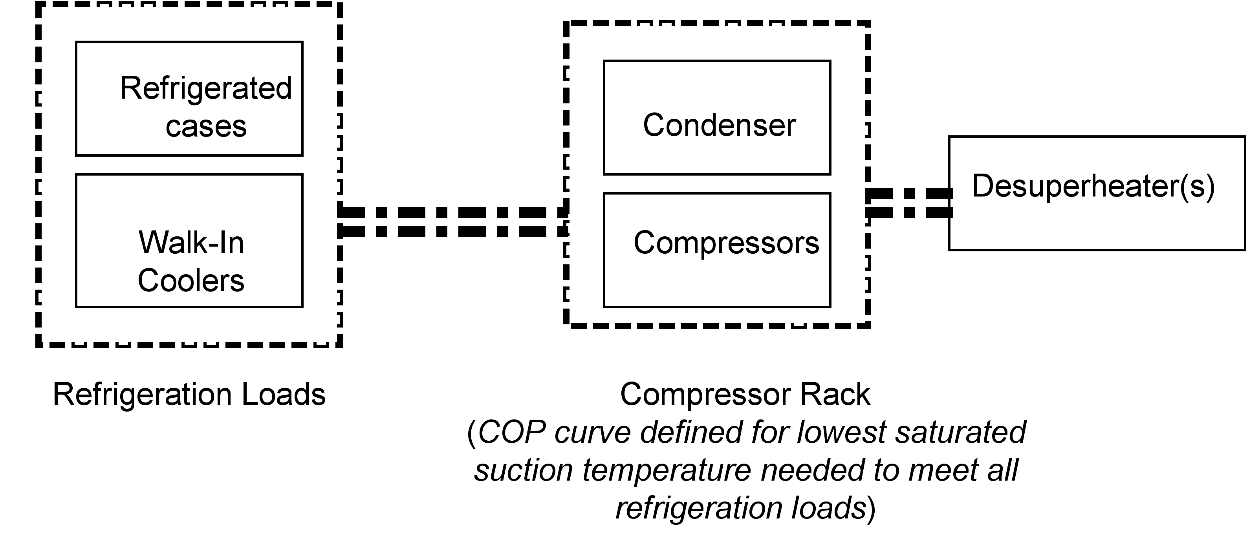
\includegraphics[width=0.9\textwidth, height=0.9\textheight, keepaspectratio=true]{media/image6091.png}
\caption{Typical Compressor Rack Equipment Schematic \protect \label{fig:typical-compressor-rack-equipment-schematic}}
\end{figure}

\begin{figure}[hbtp] % fig 277
\centering
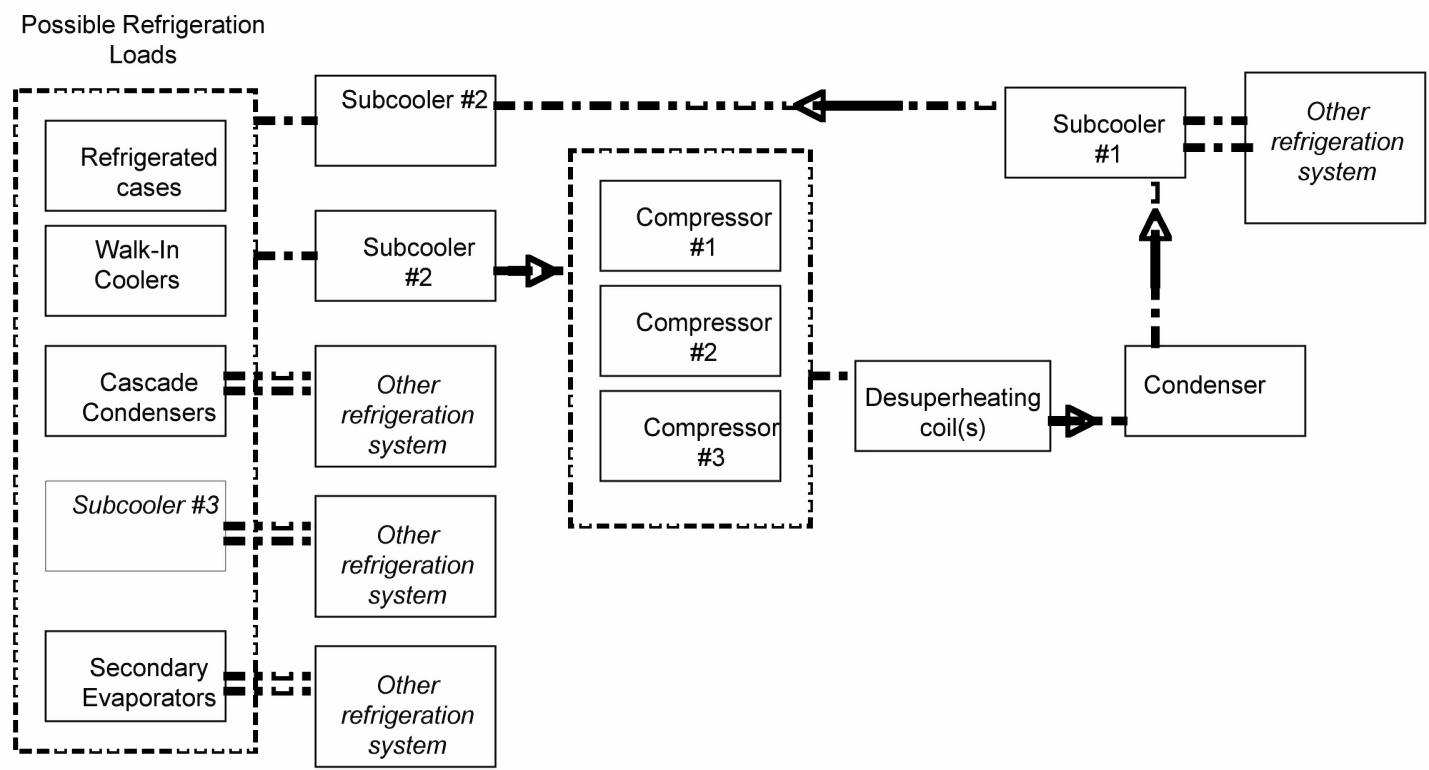
\includegraphics[width=0.9\textwidth, height=0.9\textheight, keepaspectratio=true]{media/image6092.png}
\caption{Typical Detailed Refrigeration System Equipment Schematic \protect \label{fig:typical-detailed-refrigeration-system}}
\end{figure}

Four classes of secondary refrigeration loops can be modeled:

\begin{itemize}
  \item a separate water loop is used to remove heat rejected by the condenser,
  \item a lower-temperature refrigeration system rejects heat to a higher-temperature refrigeration system via a cascade condenser,
  \item a fluid, such as a brine or glycol solution, is cooled in a secondary evaporator and is then circulated to chill the refrigerated cases and walk-ins, and
  \item a refrigerant, such as CO\(_{2}\), is partially evaporated in the refrigerated cases and walk-ins in a liquid-overfeed circuit, and then condensed in a secondary evaporator.
\end{itemize}

The first two classes of secondary loops are modeled using Refrigeration:System objects with Refrigeration:Condenser:WaterCooled and Refrigeration:Condenser:Cascade objects, respectively.~ Figure~\ref{fig:typical-detailed-refrigeration-system} shows how cascade condensers and secondary evaporators are treated as a refrigeration load on a primary detailed system. The second two classes are modeled with a Refrigeration:SecondarySystem object described later in this section.

The compressor rack, detailed and secondary refrigeration systems, refrigerated case, and other component models are described below. The optional air and water heating coils are described elsewhere in this document (Ref. objects Coil:Heating:Desuperheater and Coil:WaterHeating:Desuperheater).

\subsection{Refrigeration Compressor Racks}\label{refrigeration-compressor-racks}

The refrigerated case compressor rack object works in conjunction with the refrigerated case and walk-in cooler objects (Refrigeration:Case and Refrigeration:WalkIn) to simulate the performance of a simple supermarket-type refrigeration system. This object (Refrigeration:CompressorRack) models the electric consumption of the rack compressors and the cooling of the compressor rack's condenser. Heat removed from the refrigerated cases and walk-ins and compressor/condenser fan heat can be rejected either outdoors or to a zone. Compressor rack condenser waste heat can also be reclaimed for use by an optional air heating coil (Ref. object Coil:Heating:Desuperheater) or by a user-defined plant water loop (Ref. object Coil:WaterHeating:Desuperheater).

The performance of the compressor rack is simulated using the sum of the evaporator loads for all refrigerated cases and walk-ins connected to the rack. Whether a single refrigerated case is connected to a rack (e.g., stand-alone refrigerated case, meat cooler, or produce cooler) or several cases are connected to a rack, the rack electric consumption is calculated based on the total evaporator load for the connected cases and walk-ins and the coefficient of performance (COP) for the compressor rack. At least one refrigerated case or walk-in must be connected to the compressor rack. The model assumes the compressor rack has sufficient capacity to meet the connected refrigeration load for any simulation time step. Additionally, the model neglects compressor cycling losses at part-load conditions.

For condenser heat rejection to the outdoors, condenser cooling can be modeled as dry air cooling, wet evaporative cooling, or water loop cooling. Using evaporative cooling rather than dry air cooling will allow for more efficient condenser heat rejection based on the entering air approaching the wet-bulb temperature rather than the dry-bulb temperature. Analyses under the International Energy Agency's (IEA) Heat Pumping Programme Annex 26 indicates that this measure can improve refrigeration system efficiency by up to 10\% (IEA 2003). The use of an evaporative-cooled condenser requires a water pump and, optionally, a basin sump water heater (to protect against freezing). Makeup water will also be required to replace that lost by evaporation. In colder climates, some evaporative-cooled condensers are drained for the winter months and run as dry air units. This scenario can be modeled by using an optional evaporative condenser availability schedule.

The simulation of the evaporative cooled condenser utilizes an effective air dry-bulb temperature that is assumed to be the result of evaporation of water in the air stream (similar to object EvaporativeCooler:Direct:CelDekPad). As discussed below, this effective temperature is used by performance curves that are a function of temperature. While some designs of evaporative coolers use water film cascading across the condenser coil for evaporative cooling, the current model uses the effective temperature method as a surrogate for the more complex water film on coil calculations.

If the condenser heat rejection is specified as water cooled, an appropriate plant water loop must be defined by the user (see documentation on \emph{Plant/Condenser Loops} for additional details about plant loops).~ This will include defining cooling supply components, such as pumps, water storage tanks, and cooling towers, as well as related branches, nodes, and connectors. The heat rejection from the refrigeration condenser is modeled as a cooling demand, which is satisfied by heat extraction devices (e.g., water tank and cooling tower) on the cooling supply side of a water loop. An example of such an arrangement is shown in Figure~\ref{fig:example-of-condenser-heat-recovery-to-water}.

\begin{figure}[hbtp] % fig 278
\centering
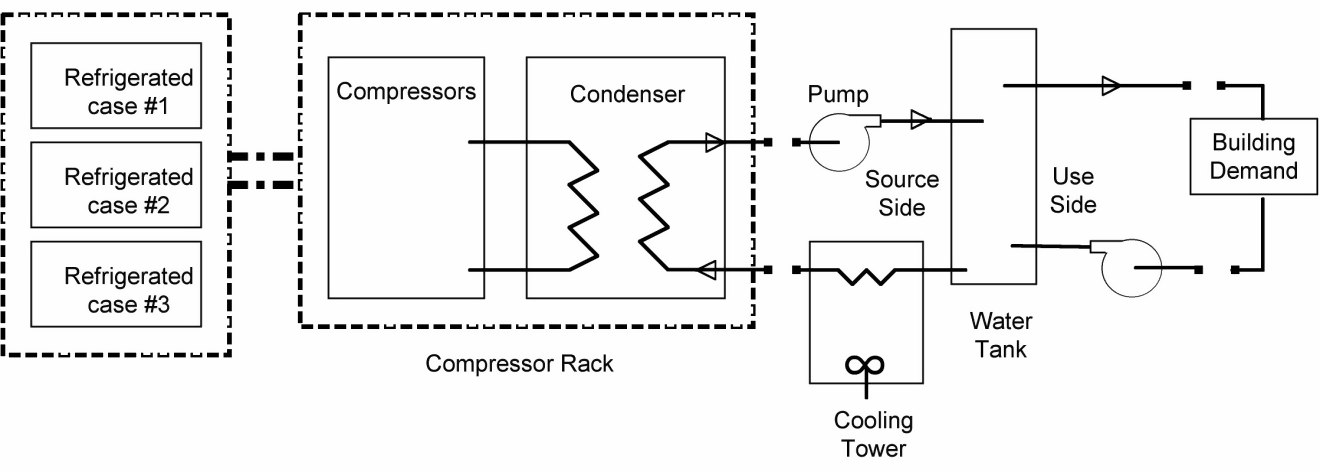
\includegraphics[width=0.9\textwidth, height=0.9\textheight, keepaspectratio=true]{media/image6093.png}
\caption{Example Of Condenser Heat Recovery To Water Storage Tank \protect \label{fig:example-of-condenser-heat-recovery-to-water}}
\end{figure}

\subsubsection{Compressor Energy Use}\label{compressor-energy-use}

Calculation of compressor rack electric power uses a simple model based on the total evaporator load (sum of the evaporator loads for all refrigerated cases and walk-ins connected to a rack) and the compressor rack operating COP which accounts for the air temperature entering the condenser:

\begin{equation}
CO{P_{operating}} = CO{P_{design}}\left( {COPfTemp} \right)
\end{equation}

where:

\(CO{P_{operating}}\) is the compressor coefficient of performance at actual operating conditions (W/W)

\(CO{P_{design}}\) is the compressor coefficient of performance at design conditions (W/W)

\(COPfTemp\) is the output of the normalized ``Compressor Rack COP as a Function of Temperature Curve'' (dimensionless).

Because the COP curve is defined only as a function of the condensing temperature, it is important that this curve definition corresponds to the lowest evaporating temperature served by the compressor rack. The air temperature used to evaluate the ``Compressor Rack COP as a Function of Temperature Curve'' depends on where the compressor rack's condenser is located (Heat Rejection Location). When modeling condenser heat rejected directly to a zone (typical of a stand-alone packaged refrigerated case with integral condenser located in a building zone), the zone air dry-bulb temperature is used to calculate the change in compressor COP from the design value. If more than one refrigerated case and no walk-ins are attached to a compressor rack that rejects its condenser heat to a zone, then all cases served by this rack must reside in the same zone. When modeling a compressor rack serving at least one walk-in, OR with condenser heat rejected to outdoors, the refrigerated cases and walk-ins connected to this rack may be located in different zones. If the condenser type is specified as ``Air Cooled'', the outdoor air dry-bulb temperature is used to evaluate the ``Compressor Rack COP as a Function of Temperature Curve.''~ If the condenser type is specified as ``Evap Cooled'', the air temperature leaving the condenser is related to the effectiveness of the evaporative cooling system. If the evaporative process were 100\% effective, the effective temperature of air leaving the evaporative media would equal the air wet-bulb temperature. However, the efficiency of the direct evaporative process is typically less than 100\%, and the effective temperature leaving the condenser is determined by:

\begin{equation}
{T_{effective}} = {T_{owb}} + (1 - \varepsilon )*[{T_{odb}} - {T_{owb}}]
\end{equation}

where:

\({T_{effective}}\) is the effective dry-bulb temperature of air leaving the condenser cooling coil (\(^{\circ}\)C)

\({T_{owb}}\) is the outdoor air wet-bulb temperature (\(^{\circ}\)C)

\({T_{odb}}\) is the outdoor air dry-bulb temperature (\(^{\circ}\)C)

\(\varepsilon\) is the evaporative condenser effectiveness.

If the user is modeling an evaporative cooled condenser and is using COPfTemp curve data (e.g., manufacturer's data) based on wet-bulb temperature rather than dry-bulb temperature, the evaporative condenser effectiveness should be set to 1.0 for consistency.

If the condenser is water cooled, the effective temperature experienced by the condenser is based on the return water temperature from the plant loop heat rejection system (e.g., cooling tower) that is defined by the user. This return water temperature is typically related to the outdoor ambient conditions at each time step.

The electric power input to the rack compressor(s) is calculated for each simulation time step as the sum of the connected refrigerated case evaporator loads divided by the operating COP:

\begin{equation}
{P_{{\rm{rack}}}} = \frac{{\sum {{{\dot Q}_{case}} + \sum {{{\dot Q}_{walkin}}} } }}{{CO{P_{operating}}}}
\end{equation}

where:

\({P_{rack}}\) is the output variable ``Refrigeration Compressor Rack Electric Power {[}W{]}'', electric power input to the rack compressor(s)

\({\dot Q_{case}}\) is the evaporator load for each refrigerated case connected to the rack (W)

\({\dot Q_{walkin}}\) is the refrigeration load for each walk-in connected to the rack (W).

\subsubsection{Condenser Heat Rejection, Energy Use, and Water Use}\label{condenser-heat-rejection-energy-use-and-water-use}

The compressor rack can reject heat to an air-, water-, or evaporative-cooled condenser. The condenser type determines the heat rejection temperature used for the compressor rack COP calculation. The compressor rack also allows superheat heat reclaim and heat rejection to a conditioned zone.

\paragraph{Condenser Fan Energy Use}\label{condenser-fan-energy-use}

Condenser fan power for any simulation time step is calculated by multiplying the design fan power by the condenser fan power as a function of temperature curve.

\begin{equation}
{P_{CondFan}}\,\, = {P_{CondFan,design}}\left( {CondFanfTemp} \right)
\end{equation}

where:

\({P_{CondFan}}\) is the output variable ``Refrigeration Compressor Rack Condenser Fan Electric Energy {[}W{]}''

\({P_{CondFan,design}}\) is the design condenser fan power (W)

\(CondFanfTemp\) is the output of the optional ``Condenser Fan Power as a Function of Temperature Curve''.

Similar to the compressor rack energy use described above, the air temperature used to evaluate the ``Condenser Fan Power as a Function of Temperature Curve'' depends on where the condenser rack's condenser is located (i.e., zone air dry-bulb temperature if the condenser is located in a zone, outdoor air dry-bulb temperature if the condenser is located outdoors and is specified as air cooled, or effective temperature if the condenser is outdoors and is specified as evaporative cooled). If the sum of the evaporator loads for the refrigerated cases connected to the rack is equal to zero, the condenser fan power is set equal to zero. If the user does not provide a ``Condenser Fan Power as a Function of Temperature Curve'', then the model assumes the condenser fan power is at the design power level when any of the refrigerated cases connected to this rack are operating.

If the user is modeling an evaporative cooled condenser and is using CondFanfTemp curve data based on wet-bulb temperature rather than dry-bulb temperature, the evaporative condenser effectiveness should be set to 1.0 for consistency.

For a water cooled condenser, there is no fan load at the condenser (i.e., the~ water/refrigerant heat exchanger). Any fan load would be related to and accounted for at the heat rejection object (e.g., cooling tower).

\paragraph{Superheat Reclaim Heating Coil}\label{superheat-reclaim-heating-coil}

EnergyPlus can simulate waste heat being reclaimed from a compressor rack for use by a refrigerant-to-air or refrigerant to water heating coil. Heat reclaimed from the compressor rack is assumed to be recovered from the superheated refrigerant gas leaving the compressor(s) and does not directly impact the performance of the compressor rack or refrigerated cases connected to the rack. The total heat rejected by the condenser (in Watts) is calculated each time step as follows:

\begin{equation}
{\dot Q_{condenser}} = \left( {\sum {{{\dot Q}_{case}} + \left. {\sum {{{\dot Q}_{walkin}}} } \right)} } \right.\left( {1 + \left. {\frac{1}{{CO{P_{operating}}}}} \right)} \right.
\end{equation}

The heat reclaim heating coil is able to transfer a fixed percentage of this total amount of rejected energy (not to exceed 30\%) and use it to heat air and water. Refer to objects Coil:Heating:Desuperheater and Coil:WaterHeating:Desuperheater for a complete description of how these coils are modeled.

NOTE: When modeling a heat reclaim coil, the heat rejection location in the Refrigeration:CompressorRack object must be ``Outdoors''. If the compressor rack heat rejection location is ``Zone'', the total amount of waste heat available for reclaim (e.g., by a desuperheater heating coil) is set to zero by the compressor rack object and the simulation proceeds.

\paragraph{Heat Rejection to Zone}\label{heat-rejection-to-zone}

The compressor rack model can simulate condenser heat being rejected to a zone. As explained previously, if this heat rejection option is selected then all refrigerated cases connected to the rack must be located in the same zone and a superheat heat reclaim heating coil can not be modeled (Ref. Superheat Reclaim Heating Coil).

The refrigerated case and walk-in objects (Refrigeration:Case and Refrigeration:WalkIn) already calculate and report the sensible case credits which impact the zone air heat balance (Ref. Sensible Case Credits). When refrigerated cases and/or walk-ins are served by a compressor rack that rejects condenser waste heat directly to the zone (e.g., a stand-alone refrigerated case with integral compressor and condenser), this condenser waste heat also impacts the zone air heat balance and offsets some or all of the sensible case credits.

If only cases are served, the amount of condenser waste heat rejected to the zone and/or the HVAC return air (zone return air path outlet node) is calculated and reported by the refrigerated case compressor rack object as follows:

\begin{equation}
{\dot Q_{Zone,heating}} = \frac{{\sum {\left( {{{\dot Q}_{case}}[1 - RAF]} \right)} }}{{\sum {\left( {{{\dot Q}_{case}}} \right)} }} \left( {{{\dot Q}_{condenser}} + {P_{CondFan}}} \right)
\end{equation}

\begin{equation}
{\dot Q_{HVAC,heating}} = \left( {{{\dot Q}_{condenser}} + {P_{CondFan}}} \right) - {\dot Q_{zone,heating}}
\end{equation}

where:

\({\dot Q_{Zone,heating}}\) is the output variable ``Refrigeration Compressor Rack Zone Sensible Heating Rate'' (W)

\emph{RAF} is the return air factor for each case connected to the rack (Ref. Figure~\ref{fig:return-air-factor-versus-under-case-hvac})

\({\dot Q_{HVAC,heating}}\) is the output variable ``Refrigeration Compressor Rack Return Air Sensible Heating Rate'' (W).

If the HVAC system is off for a simulation time step (no return air mass flow), the rack condenser heat normally attributed to the HVAC return is set equal to zero and all condenser heat energy is applied to the zone air heat balance.

If, however, walk-in cooler(s) are also served by this compressor rack, no condenser heat is rejected to the HVAC return air. For walk-in cooler(s), the user must specify the zone that accepts the condenser heat rejection (because walk-ins can exchange heat with multiple zones). In that case:

\begin{equation}
{\dot Q_{Zone,heating}} = {\dot Q_{condenser}} + {P_{CondFan}}
\end{equation}

\paragraph{Water Cooled Condenser}\label{water-cooled-condenser}

If the refrigeration condenser is water cooled, a water plant loop must be defined in the input file. At a minimum, the loop must contain a pump and one or more heat sinks of sufficient capacity to remove the condenser heat load. In the system shown in Figure~\ref{fig:example-of-condenser-heat-recovery-to-water}, the heat sinks are the water heater tank and the cooling tower. The water pump in the loop can be either constant (Ref. Pump:ConstantSpeed)~ or variable speed (Ref. Pump:VariableSpeed). A variable speed pump permits the loop flow to vary and allows for a setpoint to be established on the condenser outlet water temperature. As the refrigeration condenser heat load varies through time, the speed of the pump can be adjusted to achieve a mass flow consistent with a desired outlet water temperature according to

\begin{equation}
\dot{m} = \frac{{{Q_{condenser}}}}{{{c_p} \cdot ({T_{out}} - {T_{in}})}}
\end{equation}

where:

\emph{\(\dot{m}\)} is the mass flow in the water loop

\emph{Q\(_{condenser}\)} is the heat rejected by the condenser

\emph{c\(_{p}\)} is the specific heat of water

\emph{T\(_{out}\)} is the desired water outlet temperature

\emph{T\(_{in}\)} is the return water inlet temperature.

The desired water outlet temperature is specified using a schedule, subject to a maximum water outlet temperature (input specified). The maximum temperature is typically defined by constraints on the refrigerant loop pressures and temperatures. The desired mass flow in the water loop to meet the temperature schedule is also compared to the user-supplied maximum flow rate. If the desired mass flow is greater than the maximum allowed flow, the flow rate is set to the maximum value and the resulting water outlet temperature is determined.

The return water inlet temperature is a function of the cooling system defined by the user. A minimum return water temperature may need to be taken into consideration to prevent lowering the resulting refrigerant condensing pressure to the point that refrigerant expansion valve operation becomes impaired. When ambient conditions produce low temperature warnings based on the minimum return water temperature, an outlet temperature setpoint control may need to be placed on the water heat sink object (e.g., cooling tower) to keep the return water temperature above the minimum.

If the water loop flow is constant (i.e., driven by a constant speed pump), then the outlet water temperature will vary with the amount of heat rejected by the condenser.~~~ Using the equation above, the resulting water outlet temperature is calculated as

\begin{equation}
{T_{out}} = \frac{{{Q_{condenser}}}}{{{c_p} \cdot \dot{m}}} + {T_{in}}
\end{equation}

\paragraph{Evaporative Condenser Water Pump}\label{evaporative-condenser-water-pump}

If the condenser type is specified as ``Evap Cooled'', a water pump is required to circulate water in the evaporative condenser. The pump power can be input directly or be autocalculated using a relationship of 0.004266 W per watt {[}15 W/ton{]} of rated total cooling capacity where the total cooling capacity is the sum of the rated total cooling capacities for the refrigeration load connected to this compressor rack. Following manufacturer's recommendations regarding the avoidance of scaling, the water pump does not cycle when there is no cooling demand (i.e., when the compressors are not running), but rather runs continuously. However, if the evaporative condenser availability schedule is set such that evaporative cooling is not available (e.g., during very cold months to avoid freezing), then the pump power consumption will be zero during that period.

\paragraph{Evaporative Condenser Water Consumption}\label{evaporative-condenser-water-consumption}

With evaporative cooling of the condenser's entering air, makeup water is needed to replenish the water lost due to evaporation. The quantity required is calculated as the product of the air mass flow rate and the difference between the entering and leaving air humidity ratio, divided by the density of water. The air mass flow rate is determined by multiplying the evaporative condenser air volume flow rate times the density of the entering air (i.e., at the condenser air inlet node if provided, or outdoor air conditions {[}e.g., no adjustment for height above ground{]} if the condenser air inlet node field is left blank). The volumetric air flow rate is either specified directly in the user input or is autocalculated using the relationship 0.000144 m\(^{3}\)/s per watt of rated total cooling capacity {[}850 cfm/ton{]} where the total cooling capacity is the sum of the rated total cooling capacities for the refrigerated cases and walk-ins connected to this compressor rack (Ref. Refrigeration:Case and Refrigeration:WalkIn). The air mass flow rate is multiplied by the variable \emph{CondFanfTemp}, described above, to simulate the modulation of air flow by the condenser fans (e.g., staging, multi-speed, or variable speed) as a function of temperature. Mathematically,

\begin{equation}
{\dot V_{evaporation,makeup}} = \frac{{{{\dot m}_{air}}\left( {CondFanfTemp} \right)({\omega_{air,outlet}} - {\omega_{air,inlet}})}}{{{\rho_{water}}}}
\end{equation}

where:

\(\mathop {{{\dot V}_{evaporation,makeup}}}\limits^{}\) is the Refrigeration Compressor Rack Evaporative Condenser Water Volume Flow Rate (m\(^{3}\)/s)

\(\dot m_{air}\)  is the mass flow rate of air through the evaporative condenser (kg/s)

\({\omega_{air,outlet}}\) is the humidity ratio of air leaving the evaporative media (kg\(_{water}\)/kg\(_{dry\\ air}\)) based on the effective dry-bulb temperature \emph{T\(_{effective}\)}, as described above, outdoor air wet-bulb temperature, and outdoor barometric pressure

\({\omega_{air,inlet}}\) is the humidity ratio of inlet air (kg\(_{water}\)/kg\(_{dry\\ air}\)) based on conditions at the condenser air inlet node if provided, or outdoor air conditions (e.g., no adjustment for height above ground) if the condenser air inlet node field is left blank

\({\rho_{water}}\) is the density of water evaluated at the effective air temperature (kg/m\(^{3}\)).

The source of the makeup water may be specified as a water storage tank. If not specified, the makeup water is assumed to come from the building mains (Ref. Water Mains Temperatures).

\paragraph{Evaporative Condenser Basin Heater}\label{evaporative-condenser-basin-heater}

In cold climates, a basin heater may be needed to prevent freezing of the evaporative cooling water. This feature is included in the model whereby an electric basin heater provides heat to the sump water only when the condenser cooling system is idle (i.e., no refrigeration load) and when the outdoor air dry-bulb temperature is below a user-specified setpoint. Since heat balances and basin water temperatures are not explicitly determined, a linear loading relationship, as a function of the difference in outdoor air dry-bulb temperature and the setpoint temperature, is used calculate the power demand at a given time step by the basin heater.

\begin{equation}
{P_{basinheater}} = {P_{heatercapacity}}*({T_{setpoint}} - {T_{OutDb}})
\end{equation}

where:

\({P_{basinheater}}\) is the electric power demand for basin heater in current time step (W)

\({P_{heatercapacity}}\) is the electric heater capacity as a function of differential temperature (W/K)

\({T_{setpoint}}\) is the setpoint temperature below which the heater turns on (\(^{\circ}\)C)

\({T_{OutDb}}\) is the outdoor air dry-bulb temperature (\(^{\circ}\)C).

A default value for the basin heater capacity of 200 W/K has been established based on manufacturer data.

\paragraph{Evaporative Condenser Availability Schedule}\label{evaporative-condenser-availability-schedule}

Some manufacturer's evaporative cooling systems for refrigeration condensers permit seasonal draining in the colder months and operation as an air-cooled system during that time. This optional feature is available through an availability schedule. This is important in climates subject to freezing weather in order to avoid excessive ice formation on the condenser surfaces and surroundings. (The Availability Schedule is the correct way to model the use of evaporative condensers in cold climates. However, some users may take a single input description and use it to model a building with a refrigeration system in a variety of climates. To avoid modeling the use of evaporative coolers in freezing weather, the code includes a cutout to switch to dry operation whenever the outdoor drybulb temperature drops below 4\(^{\circ}\)C.) During periods when evaporative cooling is not available, the outdoor condenser behaves as an air-cooled system with no water consumption or pump and basin heater loads. The effective temperature of air entering the condenser coil during this period (used to evaluate COPfTemp and CondFanfTemp) is equal to the outdoor air dry-bulb temperature at the condenser air inlet node if provided, or outdoor air conditions (e.g., no adjustment for height above ground) if the condenser air inlet node field is left blank.

\subsection{Refrigerated Cases}\label{refrigerated-cases}

The refrigerated case object (Refrigeration:Case) works in conjunction with the compressor rack, detailed refrigeration system, or secondary refrigeration system object (Refrigeration:CompressorRack, Refrigeration:System, or Refrigeration:SecondarySystem) to simulate the performance of a refrigerated case system. The refrigerated case model uses performance information at rated conditions along with performance curves for latent case credits and defrost heat load to determine performance at off-rated conditions. Energy use for lights, fans and anti-sweat heaters is modeled based on inputs for nominal power, schedules, and control type. The refrigerated case model accounts for the sensible and latent heat exchange with the surrounding environment (termed ``case credits'') which impacts the temperature and humidity in the zone where the case is located. The simplified model described here provides the flexibility to simulate a broad range of refrigerated case types.

The total load on the refrigerated case evaporator is made up of various components:

\begin{equation}
{\dot Q_{case}} = {\dot Q_{walls}} + {\dot Q_{rad}} + {\dot Q_{inf,sens}} + {\dot Q_{inf,lat}} + {\dot Q_{lights}} + {\dot Q_{as}} + {\dot Q_{def}} + {\dot Q_{fan}} + {\dot Q_{restock}}
\label{eq:TotalLoadRefCaseEvaporator}
\end{equation}

where:

\({\dot Q_{case}}\) is the total load on the refrigerated case evaporator (W)

\({\dot Q_{walls}}\) is the heat transfer through case walls due to the difference between the refrigerated case operating dry-bulb temperature and the zone air dry-bulb temperature (W)

\({\dot Q_{rad}}\) is the radiant heat transfer to the refrigerated case (W)

\({\dot Q_{inf,sens}}\) is the sensible heat transfer by air infiltration to the refrigerated case through the air curtain or via door openings (W)

\({\dot Q_{inf,lat}}\) is the latent heat transfer by air infiltration to the refrigerated case through the air curtain or via door openings (W)

\({\dot Q_{lights}}\) is the lighting heat load (W)

\({\dot Q_{as}}\) is the anti-sweat heater load (W)

\({\dot Q_{def}}\) is the defrost heat load (W)

\({\dot Q_{fan}}\) is the fan heat load (W)

\({\dot Q_{restock}}\) is the sensible load on the refrigerated case due to restocking of products that are at a higher temperature than the case (W).

The model assumes that these load components are known for a refrigerated case at rated ambient air conditions (typically 23.9\(^{\circ}\)C {[}75\(^{\circ}\)F{]} and 55\% relative humidity) and the specified case operating temperature. A combination of user input curves and fixed correlations (defined within EnergyPlus) adjust for case performance at off-rated conditions. Several of the load components are typically provided by the case manufacturer (e.g., total rated load, fan, lighting, anti-sweat heater, and defrost loads). The remaining load components are not usually provided by the manufacturer and must be estimated (heat conduction through case walls, radiation heat transfer, sensible/latent air infiltration, and restocking).

For estimating the latent air infiltration load, the model requires that the user provide the latent heat ratio (LHR) for the refrigerated case at rated conditions. Research results are available to provide guidance in selecting this value (ASHRAE 2002, Howell 1993a, Howell 1993b). The rated LHR for refrigerated cases typically ranges from 0.1 to 0.3 depending on case configuration (e.g., glass door reach-in versus multi-deck open case) and case operating temperature.

The case loads due to wall heat conduction, radiation, and sensible air infiltration are estimated by the model as a single lumped value (sensible case credits). The sensible case credits are calculated by subtracting the known loads at rated conditions (fan, lighting, anti-sweat heater, defrost and latent case credits) from the rated total cooling capacity of the case which is provided by the case manufacturer (\({\dot Q_{case,rated}}\)).

Using these assumptions and the schedule inputs provided by the user, the refrigerated case evaporator load components in Equation~\ref{eq:TotalLoadRefCaseEvaporator} are determined for each simulation time step. The variation in certain loads with respect to changes in ambient air temperature and/or humidity (e.g., latent and sensible case credits, defrost load, and anti-sweat heater load) are factored into the calculation based on user-provided inputs or by the model itself.

Whenever the total heat load on the case is greater than the available evaporator capacity, such as during defrost (when the evaporator capacity is set to zero) or restocking, the load is accumulated to be met during subsequent time steps. This accounts for the energy required to bring the case back down to the rated operating temperature even though the rise in case temperature during defrost or restocking is not explicitly modeled. Following defrost, it may take multiple time steps to meet this accumulated load.

The specific calculations for case evaporator load components and electric power for these loads (as applicable) are provided below.

\subsubsection{Case Evaporator Fan}\label{case-evaporator-fan}

The refrigerated case evaporator fan electric power is calculated for each simulation time step as the product of the operating case fan power per unit length of case, the length of the refrigerated case, and the fraction of time that the case is not being defrosted. For cases with hot-gas or electric defrost (with or without temperature termination), the fan is disabled during the entire scheduled defrost drip-down time period. The evaporator fan operates continuously for off-cycle defrost or no defrost.

\begin{equation}
{P_{fan}} = {P'}_{fan,oper}\left( {{L_{case}}} \right)\left( {1 - SC{H_{defrost,dripdown}}} \right)
\end{equation}

where:

\({P_{fan}}\) is the output variable ``Refrigerated Case Evaporator Fan Electric Power {[}W{]}''

\({P'}_{fan,oper}\) is the operating case fan power per unit length (W/m)

\({L_{case}}\) is the case length (m)

\(SC{H_{defrost,dripdown}}\) is the fraction of time case is being defrosted (0 to 1), including drip-down period (based on the defrost drip-down schedule) for hot-gas or electric defrost. For off-cycle defrost or no defrost, this value is set to zero for this calculation.

The model assumes that the evaporator fan is entirely contained within the thermal envelope of the case, and that all fan power results in a direct heat load on the case evaporator:

\begin{equation}
{\dot Q_{fan}} = {P_{fan}}
\end{equation}

\subsubsection{Case Lighting}\label{case-lighting}

The refrigerated case lighting electric power is calculated for each simulation time step as the product of the installed case lighting power per unit length of case, the lighting schedule value, and the length of the refrigerated case:

\begin{equation}
{P_{lights}} = P{'_{lights,installed}}({L_{case}})(SC{H_{lights}})
\end{equation}

where:

\({P_{lights}}\) is the output variable ``Refrigerated Case Lighting Electric Power {[}W{]}''

\(P{'_{lights,installed}}\) is the installed case lighting power per unit length (W/m)

\(SC{H_{lights}}\) is the case lighting schedule value (0 to 1).

A maximum schedule value of 1.0 means the lights are fully on at the installed case lighting power level. Schedule values of 0.0 indicate the lights are off and 0.5 at half-power.

The user can specify the fraction of lighting energy that directly contributes to the case evaporator heat load:

\begin{equation}
{\dot Q_{lights}} = \,{P_{lights}}\left( {{F_l}} \right)
\end{equation}

where \({F_l}\) is the fraction of lighting energy to case.

The remainder of the lighting energy (1 - \emph{F\(_{l}\)}) is a heating load to the zone where the case is located, which is discussed further in section Sensible Case Credits below. This fraction (1 - \emph{F\(_{l}\)}) can be used to represent lighting ballasts and/or bulbs located outside the air curtain of the refrigerated case.

\subsubsection{Anti-Sweat Heater Performance}\label{anti-sweat-heater-performance}

Anti-sweat heaters warm the refrigerated case rails or doors to provide protection from moisture condensation. Different anti-sweat heater control strategies are used depending on the case temperature and the type of anti-sweat heater installed. Several types of anti-sweat heater control strategies can be simulated with this model: constant, linear variation with ambient relative humidity or dewpoint temperature, and a theoretical model that determines the minimum anti-sweat heater power required to maintain the case surface just above the temperature where condensation would occur. Additionally, anti-sweat heater performance can be disregarded if the type of refrigerated case does not warrant its use. For the control strategies described below (except ``None'' and ``Constant Method''), the model does not allow the anti-sweat heater power to be less than the minimum power nor greater than the case anti-sweat heater power specified by the user. Each anti-sweat heater control type is described in detail below.

\paragraph{None}\label{none}

Used for refrigerated cases that do not require an anti-sweat heater.

\begin{equation}
{\dot Q_{as}} = 0
\end{equation}

where \({\dot Q_{as}}\) is the anti-sweat heater load on the case evaporator (W).

\paragraph{Constant Method}\label{constant-method}

For refrigerated cases requiring constant anti-sweat heater output, the power use is simply calculated as the case anti-sweat heater power per unit length multiplied by the length of the case. This method is used when the manufacturer recommends that cycling of the heaters not occur.

\begin{equation}
{P_{as}} = {P'}_{as} \left( {{L_{case}}} \right)
\end{equation}

where:

\({P_{as}}\) is the output variable ``Refrigerated Case Anti-Sweat Heater Electric Power'' (W)

\({P'}_{as}\) is the case anti-sweat heater power per unit length (W).

\paragraph{Relative Humidity Method}\label{relative-humidity-method}

Anti-sweat heater power can be reduced at lower ambient relative humidity levels to save energy while still protecting from moisture condensation on cold surfaces. For this control type, anti-sweat heater power use is reduced linearly based on case anti-sweat heater power at the rated ambient relative humidity (typically 55\% RH), the relative humidity specified by the user where no anti-sweat heater power is required, and the relative humidity of the ambient (zone) air surrounding the case.

\begin{equation}
{P_{as}} = {P'}_{as}\left( {{L_{case}}} \right)\left( {1 - \left[ {\frac{{R{H_{rated}} - R{H_{air}}}}{{R{H_{rated}} - R{H_{\min }}}}} \right]} \right)
\end{equation}

where:

\(R{H_{air}}\) is the relative humidity of the ambient (zone) air (\%)

\(R{H_{rated}}\) is the rated ambient relative humidity (\%)

\(R{H_{\min }}\) is the relative humidity at zero anti-sweat heater energy (\%).

\paragraph{Dewpoint Method}\label{dewpoint-method}

Anti-sweat heater power can also be reduced as a function of ambient air dewpoint temperature based on a similar correlation to that used by the relative humidity method. This control method varies the anti-sweat heater power linearly based on the ambient air dewpoint temperature, the case operating temperature, and the rated ambient dewpoint temperature (calculated by the model using the rated ambient temperature and rated ambient relative humidity entered by the user).

\begin{equation}
{P_{as}} = {P'}_{as}\left( {{L_{case}}} \right)\left( {\frac{{{T_{dp,air}} - {T_{case}}}}{{{T_{dp,rated}} - {T_{case}}}}} \right)
\end{equation}

where:

\({T_{dp,air}}\) is the dewpoint temperature of the ambient (zone) air (\(^{\circ}\)C)

\({T_{dp,rated}}\) is the rated ambient dewpoint temperature (\(^{\circ}\)C)

\({T_{case}}\) is the case operating temperature (\(^{\circ}\)C).

\paragraph{Heat Balance Method}\label{heat-balance-method}

A theoretical model may also be used to simulate the performance of anti-sweat heater operation at various indoor dewpoint temperatures (Henderson and Khattar 1999). The model calculates that amount of heat required to hold the case or door surface at (or slightly above) the dewpoint temperature of the ambient air using the following simple heat balance equation:

\begin{equation}
{P_{as}} = \,\,\left( {\frac{{\left( {{T_{dp,air}} - {T_{db,air}}} \right){H_{case}}}}{{{R_{air}}}} + \frac{{\left( {{T_{dp,air}} - {T_{case}}} \right){H_{case}}}}{{{R_{case}}}}} \right){L_{case}}
\end{equation}

where:

\({T_{dp,air}}\) is the dewpoint temperature of the ambient (zone) air (\(^{\circ}\)C)

\({T_{db,air}}\) is the dry-bulb temperature of the ambient (zone) air (\(^{\circ}\)C)

\({H_{case}}\) is the height of the case (m)

\({R_{air}}\) is the air film resistance (assumed constant at 0.3169 m\(^{2}\)-\(^{\circ}\)C/W)

\({R_{case}}\) is the heat transfer resistance of case (m\(^{2}\)-\(^{\circ}\)C/W)

\({T_{case}}\) is the case operating temperature (\(^{\circ}\)C)

\({L_{case}}\) is the case length (m).

The model above provides a linear relationship of anti-sweat heater power with varying ambient air dewpoint temperature at constant ambient air dry-bulb and case temperatures. By assuming that the `nominal' anti-sweat heater power entered by the user is required to avoid moisture condensation at rated ambient air conditions, the value of \({R_{case}}\) can be determined by rearranging the equation and solving as follows:

\begin{equation}
{R_{case}} = \frac{{\left( {{T_{dp,rated}} - {T_{case}}} \right)}}{{\left( {\frac{{{P'}_{as}}}{{{H_{case}}}}} \right) - \left( {\frac{{{T_{dp,rated}} - {T_{db,rated}}}}{{{R_{air}}}}} \right)}}
\end{equation}

where \({T_{db,rated}}\) is the rated ambient temperature (\(^{\circ}\)C)

With \emph{R\(_{case}\)} known, \emph{P\(_{as}\)} can be calculated for each simulation time step using the actual ambient (zone) air dry-bulb and dewpoint temperatures.

\paragraph{All Anti-Sweat Heater Control Methods}\label{all-anti-sweat-heater-control-methods}

For all control methods, the user can specify the fraction of anti-sweat heater energy that directly contributes to the case evaporator heat load:

\begin{equation}
{\dot Q_{as}} = {P_{as}}\left( {{F_{as}}} \right)
\end{equation}

where \({F_{as}}\) is the fraction of anti-sweat heater energy to case.

The remainder of the anti-sweat heater energy (1 - \emph{F\(_{as}\)}) is a heating load to the zone where the case is located, which is discussed further in section Sensible Case Credits below.

\subsubsection{Case Restocking}\label{case-restocking}

The impact of restocking the refrigerated case with product that is not at the case operating temperature is modeled with the case restocking schedule. The schedule is entered as a heat gain rate per unit length of the refrigerated case (W/m). The heat load due to restocking is calculated as the scheduled load multiplied by the length of the refrigerated case. The load due to product restocking is assumed to be only sensible (temperature) heat; a latent (moisture) component is not modeled.

\begin{equation}
{\dot Q_{restock}} = SC{H_{restock}}\left( {{L_{case}}} \right)
\end{equation}

where \(SC{H_{restock}}\) is the refrigerated case restocking schedule value (W/m).

The restocking heat load is removed by the refrigerated case evaporator any time the case is not being defrosted and excess sensible cooling capacity is available. If the evaporator cooling capacity is insufficient to remove the entire restocking load, the unmet portion is carried over to the next simulation time step.

\subsubsection{Case Defrost}\label{case-defrost}

Eight refrigerated case defrost strategies can be simulated: none, off-cycle, electric, electric with temperature termination, hot-gas, hot-gas with temperature termination, hot-brine, and hot-brine with temperature termination. Some research has shown that the defrost times for cases defrosted using hot brine can be significantly shorter than defrost times for electric or hot gas.(Terrell, W. J. Jr., 1999) For each of these strategies, the refrigerated case evaporator is turned off for the required time period to allow accumulated frost to melt. Additional time can be scheduled (drip-down) to allow the water to drip from the evaporator and drain from the case.

Refrigerated cases typically require a specific number of defrost cycles per day for a pre-determined length of time. Refer to manufacturer's recommendations for proper defrost frequency and duration. For example, a refrigerated case may have a single defrost period each day with defrost scheduled from 7:00 -- 7:40 am and defrost drip-down scheduled from 7:00 -- 7:55 am. Notice the drip-down schedule and the defrost schedule start at the same time, and the drip-down schedule is longer than the defrost schedule. These schedules should normally repeat for each day of the year.

For electric, hot gas, and hot brine defrost types, energy use by the defrost heater occurs during the scheduled defrost period. For defrost with temperature termination, the energy is also multiplied by the defrost ratio simulating a defrost duration shorter than the defined (maximum) period. For all non-electric defrost types, defrost electric power is set equal to zero (and is not available as an output variable). For hot gas and hot brine defrost types in cases served by a detailed system, the condenser heat rejection load is reduced by the amount of heat recovered for use in the defrost system. This condenser credit is not applied for the simple compressor rack system.

If DefrostType is electric, then:

\begin{equation}
  P_{def} = {P'}_{def} L_{case} SCH_{defrost} 
\end{equation}

Else if DefrostType is ElectricWithTempTermination, then:

\begin{equation}
  P_{def} = {P'}_{def} L_{case} SCH_{defrost} \PB{DefrostRatio}
\end{equation}

Otherwise:

\begin{equation}
  P_{def} = 0.0
\end{equation}

where:

\({P_{def}}\) is the output variable ``Refrigerated Case Defrost Electric Power'' (W)

\({P'}_{def}\) is the case defrost power per unit length (W)

\({L_{case}}\) is the case length (m)

\(SC{H_{defrost}}\) is the case defrost schedule value (0 to 1)

\(DefrostRatio\) is the fraction of maximum defrost time, used with temperature termination.

Frost accumulation on the case evaporator will vary with the humidity level in the ambient air surrounding the case. Therefore, defrost heater operation can be reduced when ambient air humidity levels are low. Several methods are used to reduce unnecessary defrost heater operation, including terminating heater operation when the measured evaporator temperature indicates that the accumulated frost has been completely melted. For modeling refrigerated cases with temperature-terminated defrost, EnergyPlus allows the user to specify a defrost energy correction curve to account for variations in defrost energy as ambient air humidity levels change. The user can select from four correction curve types: None, Case Temperature Method, Relative Humidity Method, or Dewpoint Method.

For type None (default):

\begin{equation}
  DefrostRatio = 1
\end{equation}

For type Case Temperature Method:

\begin{equation}
  DefrostRatio = 1 - \PB{RH_{rated} - RH_{air}} \PB{a + b T_{case} + c T_{case}^2 + d T_{case}^3}
\end{equation}

For type RH Method:

\begin{equation}
  DefrostRatio = e + f \PB{RH_{air}} + g \PB{RH_{air}^2} + h \PB{RH_{air}^3}
\end{equation}

For type Dewpoint Method:

\begin{equation}
  DefrostRatio = i + j T_{dp,air} + k T_{dp,air}^2 + l T_{dp,air}^3
\end{equation}

where:

\(R{H_{rated}}\) is the rated ambient relative humidity (\%)

\(R{H_{air}}\) is the relative humidity of the ambient (zone) air (\%)

\({T_{case}}\) is the case operating temperature (\(^{\circ}\)C)

\({T_{dp,air}}\) is the dewpoint temperature of the ambient (zone) air (\(^{\circ}\)C)

\emph{a,~\ldots{},~l} is the user-defined coefficients using a cubic curve object (Curve:Cubic).

The user specifies the defrost energy correction curve type and the name of the cubic curve object (Curve:Cubic) that defines the curve coefficients. Representative curve coefficients for curve type ``Case Temperature Method'' are provided in Table~\ref{table:representative-defrost-energy-correction}.

% table 75
\begin{longtable}[c]{p{1.5in}p{2.36in}p{2.13in}}
\caption{Representative Defrost Energy Correction Curve Coefficients for Case Temperature Method \label{table:representative-defrost-energy-correction}} \tabularnewline
\toprule 
Coefficient & Single-shelf horizontal display case & Multi-shelf vertical display case \tabularnewline
\midrule
\endhead

a & 2.3632E-2 & 2.4598E-2 \tabularnewline
b & 6.2320E-4 & 7.6439E-4 \tabularnewline
c & 2.8320E-5 & -3.8637E-5 \tabularnewline
d & 4.4035E-7 & 7.45686E-7 \tabularnewline
\midrule
\multicolumn{3}{l}{Note: Coefficients derived for \emph{RH\(_{rated}\)} = 55\% and a rated} \tabularnewline
\multicolumn{3}{l}{ambient temperature of 23.9\(^{\circ}\)C (75\(^{\circ}\)F). Source:~ Howell 1993b.} \tabularnewline
\bottomrule
\end{longtable}

As mentioned above, the refrigerated case evaporator is turned off while it is being defrosted. Heat gains during defrost must be removed once the defrost period (drip-down schedule) has ended. The model assumes that heat gains due to defrost heater operation are at least partially offset by converting accumulated frost to liquid water (condensate) which drains from the case. Frost accumulation during each simulation time step is estimated by the model using the actual latent heat transfer to the refrigerated case and the heat of vaporization plus the heat of fusion for water. The model assumes that frost is not accumulated on the evaporator during the defrost drip-down time period.

\begin{equation}
Frost = Frost + \left( {\frac{{{{\dot Q}_{case,rated}}\left( {{L_{case}}} \right)\left( {RT{F_{rated}}} \right)\left( {LH{R_{rated}}} \right)\left( {LatentRatio} \right)\left( {{t_{zn}}} \right)}}{{\left( {{h_f} + {h_{fg}}} \right)}}} \right)\left( {1 - SC{H_{defrost,dripdown}}} \right)
\end{equation}

where:

\(Frost\)is the amount of accumulated frost on the case evaporator (kg)

\({\dot Q_{case,rated}}\) is the case rated total cooling capacity per unit length (W/m)

\({L_{case}}\) is the case length (m)

\(RT{F_{rated}}\) is the runtime fraction of the refrigerated case at rated conditions

\(LH{R_{rated}}\) is the latent heat ratio of the refrigerated case at rated conditions

\(LatentRatio\) is the ratio of actual latent load to rated latent load on the case, based on latent case credit curve (see section Latent Case Credits below)

\({t_{zn}}\) is the duration of zone simulation time step (s)

\({h_{fg}}\) is the heat of vaporization of water (assumed constant at 2,498,000 J/kg)

\({h_f}\) is the heat of fusion of water (335,000 J/kg)

\(SC{H_{defrost,dripdown}}\) is the defrost drip-down schedule value (0 to 1).

During defrost (SCHdefrost), the model assumes that the hot gas, hot brine, or electric heater energy directly contributes to melting the frost (heat of fusion of water). Defrost energy not attributed to melting frost from the evaporator coil results in a heat load on the refrigerated case evaporator (\({\dot{Q}_{def}}\)). When the defrost drip-down time period ends, this defrost energy heat load is added to the actual case load (up to the maximum evaporator capacity) until the total defrost energy heat load is removed (which may take several simulation time steps).

If DefrostType is Electric, HotGas, or HotBrine, then:

\begin{equation}
  \dot{Q}_{def} = \max\RB{0.0,\PB{P_{def}' L_{case} SCH_{def} - \frac{Frost\PB{h_f}}{t_{zn}}}}
\end{equation}

Otherwise:

\begin{equation}  
  \dot{Q}_{def} = 0.0
\end{equation}

where \({\dot Q_{def}}\) is the defrost heat load (W).

\subsubsection{Sensible Case Credits}\label{sensible-case-credits}

Refrigerated cases remove sensible energy from the surrounding environment (termed ``sensible case credits''). In this model, the sensible case credits are composed of wall heat conduction, radiation heat transfer, and sensible heat transfer by air infiltration (\({\dot Q_{walls}}\) + \({\dot Q_{rad}}\) + \({\dot Q_{{\rm{inf,sens}}}}\) in Equation~\ref{eq:TotalLoadRefCaseEvaporator}). To quantify this energy transfer, the model first calculates the rated sensible case credits by subtracting the known loads at rated conditions (fan, lighting, and anti-sweat heater) from the rated sensible cooling capacity of the case. It should be noted that the lighting and fan heat discussed here are for standard-efficiency equipment. Manufacturers typically provide ratings for both standard and high-efficiency fan and lighting equipment; however, the standard equipment is used to determine rated sensible case credits. (Some manufacturers no longer include any lighting in their rated capacity values. For these cases, P'\(_{lights,std}\) will equal zero.)

\begin{equation}
\dot Qc{c_{sens,rated}} = \left[ {{{\dot Q}_{case,rated}}\left( {RT{F_{rated}}} \right)\left( {1 - LH{R_{rated}}} \right) - {P'}_{lights,std}\left( {{F_l}} \right) - {P'}_{as}\left( {{F_{as}}} \right) - {P'}_{fan,std}} \right]{L_{case}}
\end{equation}

where:

\(\dot Qc{c_{sens,rated}}\) is the sensible case credits at rated conditions (W)

\({\dot Q_{case,rated}}\) is the case rated total cooling capacity per unit length (W/m)

\(RT{F_{rated}}\) is the runtime fraction of the refrigerated case at rated conditions

\(LH{R_{rated}}\) is the latent heat ratio of the refrigerated case at rated conditions

\({P'}_{lights,std}\) is the standard case lighting power per unit length (W/m)

\({F_l}\) is the fraction of lighting energy to case

\({P'}_{as}\) is the case anti-sweat heater power per unit length (W)

\({F_{as}}\) is the fraction of anti-sweat heater energy to case

\({P'}_{fan,std}\) is the standard case fan power per unit length (W/m)

\({L_{case}}\) is the case length (m).

For every simulation time step, the rated sensible case credits are then adjusted to account for variations at off-rated ambient air temperatures. The model also allows the user to define a case credit fraction using a schedule object. This case credit fraction can be useful for modeling cases that operate differently during specific time periods. For example, metal or plastic coverings may be installed on refrigerated display cases during unoccupied hours which would significantly reduce case credits (e.g., air infiltration) compared to occupied hours when the coverings are removed. If the user does not define a case credit fraction schedule, then the fraction is assumed to be 1 for the entire simulation.

\begin{equation}
\dot Qc{c_{sens}} = \dot Qc{c_{sens,rated}}\left( {\frac{{{T_{db,air}} - {T_{case}}}}{{{T_{db,rated}} - {T_{case}}}}} \right)\left( {SC{H_{cc}}} \right)
\end{equation}

where:

\(\dot Qc{c_{sens}}\) is the sensible case credits adjusted for ambient temperature and case credit fraction (W)

\({T_{db,air}}\) is the dry-bulb temperature of the ambient (zone) air (\(^{\circ}\)C)

\({T_{case}}\) is the case operating temperature (\(^{\circ}\)C)

\({T_{db,rated}}\) is the rated ambient (zone) dry-bulb temperature (\(^{\circ}\)C)

\(SC{H_{cc}}\) is the case credit fraction (schedule value, 0 to 1).

The sensible case credits calculated above are considered heat loads on the refrigerated case evaporator. The \textbf{\emph{net}} impact of the case credits on the surrounding zone includes adjustment for the portion of the lighting and anti-sweat heater power that does \emph{not} directly contribute to the case evaporator load. Sensible case credits are negative values when heat is removed from the zone load.

\begin{equation}
\dot Qc{c_{sens,NET}} = {P_{lights}}(1 - {F_l})\,\, + \,\,{P_{as}}(1 - {F_{as}})\,\, - \,\,\dot Qc{c_{sens}}
\end{equation}

where:

\(\dot Qc{c_{sens,NET}}\) is the net impact of the sensible case credits on the surrounding zone, negative for cooling (W)

\({P_{lights}}\) is the case lighting electric power (W)

\({F_l}\) is the fraction of lighting energy to case

\({P_{as}}\) is the anti-sweat heater electric power (W)

\({F_{as}}\) is the fraction of anti-sweat heater energy to case.

When refrigerated cases are served by a compressor rack that rejects condenser waste heat directly to the zone (e.g., a stand-alone refrigerated case with integral compressor and condenser), this condenser waste heat offsets some or all of the sensible case credits. The amount of condenser waste heat rejected to the zone is calculated and reported by the refrigerated case compressor rack object (Ref. Heat Rejection to Zone).

\subsubsection{Latent Case Credits}\label{latent-case-credits}

Refrigerated cases also remove latent energy (moisture) from the surrounding environment (termed ``latent case credits''). In this model, the latent case credit is composed solely of the latent heat transfer by air infiltration \({\dot Q_{inf,lat}}\) in Equation~\ref{eq:TotalLoadRefCaseEvaporator}. The latent case credits are calculated as the product of the case length and the total cooling capacity per unit length, latent heat ratio, and runtime fraction at rated conditions. As described previously (Ref. Sensible Case Credits), a case credit fraction schedule is used to model cases that operate differently during specific time periods. The same case credit fraction is used to modify both the sensible and latent case credits. If the user does not define a case credit fraction schedule, then the fraction is assumed to be 1 for the entire simulation. The calculation of latent case credits also includes a factor (\emph{LatentRatio}) that accounts for lower ambient humidity levels. Latent case credits are set to zero during the defrost-dripdown periods.

\begin{equation}
{\dot Q_{inf,lat}} = \,\,\,\, - \dot Qc{c_{lat}}\,\, = \,\,{\dot Q_{case,rated}}\left( {LH{R_{rated}}} \right)\left( {RT{F_{rated}}} \right)\left( {SC{H_{cc}}} \right)\left( {LatentRatio} \right){L_{case}}
\end{equation}

where:

\({\dot Q_{inf,lat}}\) is the latent load on the refrigerated case evaporator at current ambient conditions (W)

\(\dot Qc{c_{lat}}\) is the latent case credit impact on zone load, negative for dehumidification (W)

\({\dot Q_{case,rated}}\) is the case rated total cooling capacity per unit length (W/m)

\(LH{R_{rated}}\) is the latent heat ratio of the refrigerated case at rated conditions

\(RT{F_{rated}}\) is the runtime fraction of the refrigerated case at rated conditions

SCH\(_{CC}\) is the case credit fraction (schedule value, 0 to 1)

\(LatentRatio\) is the ratio of actual latent load to rated latent load on the case, based on latent case credit curve

\({L_{case}}\) is the case length (m).

Latent load on the refrigerated case evaporator will vary with ambient humidity levels. Therefore, the refrigerated case model allows the user to specify a latent case credit curve to adjust case credits based on ambient humidity, and the user can select from three curve types: Case Temperature Method, Relative Humidity Method, or Dewpoint Method.

If CurveType is Case Temperature Method:

\begin{equation}
  LatentRatio = 1-\PB{RH_{rated}-RH_{air}}\PB{m+nT_{case}+oT_{case}^2+pT_{case}^3}
\end{equation}

Else if CurveType is RH Method:

\begin{equation}
  LatentRatio = q + r\PB{RH_{air}} + s\PB{RH_{air}^2} + t\PB{RH_{air}^3}
\end{equation}

Else if CurveType is Dewpoint Method:

\begin{equation}
  LatentRatio = u + vT_{dp,air} + wT_{dp,air}^2 + xT_{dp,air}^3
\end{equation}

where:

\(R{H_{rated}}\) is the rated ambient relative humidity (\%)

\(R{H_{air}}\) is the relative humidity of the ambient (zone) air (\%)

\({T_{case}}\) is the case operating temperature (\(^{\circ}\)C)

\({T_{dp,air}}\) is the dewpoint temperature of the ambient (zone) air (\(^{\circ}\)C)

\emph{m,~\ldots{},~x} is the user-defined coefficients using a cubic curve object (Curve:Cubic).

The user specifies the latent case credit curve type and the name of the cubic curve object (Curve:Cubic) that defines the curve coefficients. Representative curve coefficients for curve type ``Case Temperature Method'' are provided in Table~\ref{table:representative-latent-case-credit-curve}.

% table 76
\begin{longtable}[c]{p{1.5in}p{2.36in}p{2.13in}}
\caption{Representative Latent Case Credit Curve Coefficients for Case Temperature Method \label{table:representative-latent-case-credit-curve}} \tabularnewline
\toprule 
Coefficient & Single-shelf horizontal & Multi-shelf vertical \tabularnewline
\midrule
\endfirsthead

\caption{Representative Latent Case Credit Curve Coefficients for Case Temperature Method} \tabularnewline
\toprule 
Coefficient & Single-shelf horizontal & Multi-shelf vertical \tabularnewline
\midrule
\endhead

m & 2.0376E-2 & 2.6520E-2 \tabularnewline
n & 2.4378E-4 & 1.0780E-3 \tabularnewline
o & 1.1400E-5 & -6.0256E-5 \tabularnewline
p & 1.8110E-7 & 1.2373E-6 \tabularnewline
\midrule
\multicolumn{3}{l}{Note: Coefficients derived for \emph{RH\(_{rated}\)} = 55\% and a rated} \tabularnewline
\multicolumn{3}{l}{ambient temperature of 23.9\(^{\circ}\)C (75\(^{\circ}\)F). Source:~ Howell 1993b.} \tabularnewline
\bottomrule
\end{longtable}

\subsubsection{Refrigerated Case Credits With Under Case Return Air}\label{refrigerated-case-credits-with-under-case-return-air}

For certain refrigerated case types, the sensible case credits provided to the zone can create an uncomfortably cold environment in the surrounding area. For this reason, return air ducts are frequently placed behind these cases to draw this cold air under the case and direct it back to the HVAC system. This reduces localized over-cooling and improves occupant comfort.

\begin{figure}[hbtp] % fig 279
\centering
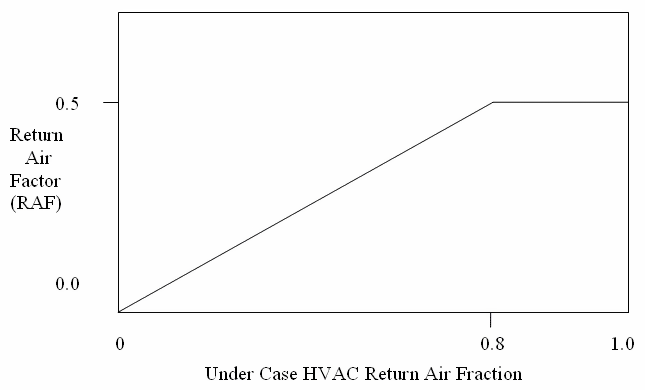
\includegraphics[width=0.9\textwidth, height=0.9\textheight, keepaspectratio=true]{media/image6247.png}
\caption{Return Air Factor Versus Under Case HVAC Return Air Fraction \protect \label{fig:return-air-factor-versus-under-case-hvac}}
\end{figure}

Since under case return ducts reduce the temperature and humidity of the air being recirculated to the HVAC system, this can impact HVAC system performance. Figure~\ref{fig:return-air-factor-versus-under-case-hvac} shows the relationship that is used by the refrigerated case model to determine the fraction of case credits that directly cool and dehumidify the HVAC system return air. This fraction, referred to as the Return Air Factor (RAF), is a function of the fraction of the HVAC system return air that comes from under the cases. The remaining fraction of the case credits (1-RAF) becomes part of the overall zone air energy balance. If the HVAC system is off for a simulation time step (no return air mass flow), the sensible and latent case credits normally attributed to the HVAC return are set equal to zero (even though they get calculated and reported here as non-zero values) and all case credit energy is applied to the zone air heat balance.

\begin{equation}
\dot Qc{c_{sens,zone}} = \dot Qc{c_{sens,NET}}\left( {1 - RAF} \right)
\end{equation}

\begin{equation}
\dot Qc{c_{lat,zone}} = \dot Qc{c_{lat}}\left( {1 - RAF} \right)
\end{equation}

\begin{equation}
\dot Qc{c_{sens,HVAC}} = \dot Qc{c_{sens,NET}}\left( {RAF} \right)
\end{equation}

\begin{equation}
\dot Qc{c_{lat,HVAC}} = \dot Qc{c_{lat}}\left( {RAF} \right)
\end{equation}

where:

\(\dot Qc{c_{sens,zone}}\) is the sensible case credit applied to the zone air heat balance (W)

\(\dot Qc{c_{lat,zone}}\) is the latent case credit applied to the zone air heat balance (W)

\(\dot Qc{c_{sens,HVAC}}\) is the sensible case credit applied to the HVAC return air (zone return air path outlet node) (W)

\(\dot Qc{c_{lat,HVAC}}\) is the latent case credit applied to the HVAC return air (zone return air path outlet node) (W)

RAF is the return air factor (see Figure~\ref{fig:return-air-factor-versus-under-case-hvac} above).

\subsubsection{Variable Evaporator Temperature}\label{variable-evaporator-temperature}

Control systems are now available that increase the evaporator temperature to improve compressor efficiency whenever the total loads on a system are less than the system capacity. To model these systems, a variable evaporator temperature is an option available with the detailed refrigeration system object (Refrigeration:System). If this option is selected, the model will compare the refrigeration load on each case to the load at rated conditions. If the case load in a particular time step is less than the rated load, an acceptable elevated evaporator temperature is determined for that case. The evaporator temperature for the whole refrigeration system is then set by the minimum evaporator temperature needed for any particular case.

\begin{equation}
  LF_{case} = \frac{\dot{Q}_{case,actual}}{\dot{Q}_{case,rated}}
\end{equation}

\begin{equation} 
  T_{Evap,Allowed} = T_{case} - LF_{case}\PB{T_{case} - T_{Evap,Design}}
\end{equation}

where:

\(LF_{case}\) is the load factor for a particular case

\(T_{Evap}\) is the evaporator temperature (\(^{\circ}\)C).

\subsection{Walk-In Coolers and Freezers}\label{walk-in-coolers-and-freezers}

The walk-in object (Refrigeration:WalkIn) is another type of refrigeration load that can be placed on either a refrigeration compressor rack, detailed refrigeration system, or secondary refrigeration system object (Refrigeration:CompressorRack, Refrigeration:System, or Refrigeration:SecondarySystem). Walk-in coolers and freezers differ from refrigerated cases in that they may have surfaces facing more than one zone and in that they are always equipped with doors, that is, they do not have open shelves. Their sensible and latent exchange with zones is therefore calculated in a different manner than for refrigerated cases. Also, the walk-in model does not interact directly with the HVAC system, that is, the return air fraction option available in the refrigerated case model is not included.

The walk-in cooler performance is based on the ASHRAE load model, which includes infiltration through door openings and sensible loss through walls/ceilings described by the user for each zone.(ASHRAE 2006d, ASHRAE 2006e, Gosney, W.B., Olama, G.A.-L. 1975) All equipment loads (fan, light, heaters) are modeled as well.~ Sensible and latent exchange with multiple adjoining zones is included. A master schedule is used for the Walk In operation and~ additional schedules control the lights, defrost, and heater operation. ~Just as for cases, unmet refrigeration loads are accumulated to be met the following time step.~ This usually occurs during defrost and ~restocking.

\subsubsection{Walk-In Sensible and Latent Heat Exchange}\label{walk-in-sensible-and-latent-heat-exchange}

A walk-in can exchange both sensible and latent energy with multiple zones.~ The heat transfer calculations are performed separately for each zone so that the heat transfer impact, or zone credits, can be determined. The area of all walls and ceilings facing each zone are described by the user by their thermal conductance and area. Sensible energy exchange takes place between these surfaces and the surrounding zones.~ Because these walls interface with conditioned zones at relatively constant temperatures, this heat exchange is modeled very simply:

\begin{equation}
Q_{SurfacesZn} = U_{SurfacesZn} \cdot A_{SurfacesZn} \cdot \Delta T_{Zn}
\end{equation}

\begin{equation}
Q_{DoorSensZn} = U_{DoorZn} \cdot Area_{DoorZn} \cdot \Delta T_{Zn}
\end{equation}

The heat transfer through the floor is similarly modeled.

\begin{equation}
Q_{Floor} = A_{Floor} x U_{Floor} x (T_{Ground} - T_{WalkIn})
\end{equation}

Where:

\(A_{Floor}\) is the area of the walkin floor (m\(^{2}\))

\(A_{SurfacesZn}\) is the area of surfaces facing Zone n (m\(^{2}\))

\(Q_{DoorSensZn}\) is the sensible heat transfer through the closed door(s) facing Zone n (W)

\(Q_{surfacesZn}\) is the sensible heat transfer through walls and ceilings facing Zone n (W)

\(T_{Ground}\) is the ground temperature (\(^{\circ}\)C)

\(T_{WalkIn}\) is the walk-in operating temperature (\(^{\circ}\)C)

\(U_{Floor}\) is the thermal conductance of floor (W/m\(^{2}\)-K)

\(U_{DoorZn}\) is the thermal conductance of doors facing Zone n (W/m\(^{2}\)-K)

\(U_{SurfacesZn\\}\) is the thermal conductance of surfaces facing Zone n (W/m\(^{2}\)-K)

\(\Delta T_{Zn}\) is the difference between walk-in operating temperature and Zone n drybulb temperature (\(^{\circ}\)C).

Infiltration through doorways places both a sensible and a latent load upon the walk-in, and corresponding credits upon the adjacent zone.~ Two types of doors are available, nominally called `stock' and `glass' doors, to enable the user to model doors that differ in thermal conductance, door protection type, and frequency of opening.~ The sensible and latent infiltration loads are modeled according to the guidance specified in (ASHRAE 2006d, ASHRAE 2009, and Gosney and Olama, 1975).~ The air within the cooler is assumed to be at 90\% relative humidity. Equal air exchange is assumed, that is, the mass of dry air infiltrating into the walkin is assumed to equal the mass of dry air infiltrating out of the walkin.

\begin{equation}
Q_{Infiltration} = Q_{FullFlow} \cdot Factor_{DoorOpen} \cdot Factor_{Flow} \cdot (1 - Factor_{Protection})
\end{equation}

\begin{equation}
Q_{FullFlow} = 0.221*A_{Door}(h_{ZoneAir}-h_{AirWalkIn})\rho_{AirWalkIn}(1-\rho_{ZoneAir}/\rho_{AirWalkIn})^{0.5}(g*H_{Door})^{0.5}Factor_{Density}
\end{equation}

\begin{equation}
Factor_{Density} = (2 /(1 + (\rho_{AirWalkIn} / \rho_{ZoneAir})^{0.333}))^{1.5}
\end{equation}

\begin{equation}
m_{DryAir} = Q_{Infiltration} / (h_{ZoneAir} - h_{AirWalkIn})
\end{equation}

\begin{equation}
m_{Water} = m_{DryAir} \cdot (W_{ZoneAir} - W_{AirWalkIn})
\end{equation}

\begin{equation}
Q_{WalkInLatentZn} = m_{Water} \cdot \Delta h_{IcetoVapor} \cdot (1 - SCH_{Defrost,DripDown})
\end{equation}

\begin{equation}
Q_{WalkInSensInfZn} = Q_{Infiltration} - (m_{Water} \cdot \Delta h_{IcetoVapor})
\end{equation}

where:

A\(_{door}\) is the area of door facing Zone n (m\(^{2}\))

Factor\(_{DoorOpen}\) is the value scheduled by user, fraction of time door open during time step

Factor\(_{Flow}\) is the doorway flow factor, = 0.8 if \(\Delta T_{Zn} \geq\) 11\(^{\circ}\)C; = 1.1 if ΔT\(\Delta T_{Zn}\) \textless{} = 11\(^{\circ}\)C

Factor\(_{Protection}\) is the doorway protection factor, = 0 for no protection; = 0.5 for an air curtain; and 0.9 for a strip curtain

g is the gravitational constant

h\(_{AirWalkIn}\) is the enthalpy of the air within the walk in, = f(T\(_{WalkIn}\),P\(_{Outdoor}\), 90\%RH) (J/kg)

h\(_{ZoneAir}\) is the enthalpy of the air in Zone n (J/kg)

H\(_{door}\) is the height of door facing Zone n (m)

Q\(_{FullFlow}\) is the sensible and latent refrigeration load for fully established flow (W)

Q\(_{Infiltration}\) is the average infiltration (sensible and latent) refrigeration load for the time step (W)

Q\(_{WalkInLatentZn}\) is the latent load upon the walk in facing Zone n (W)

Q\(_{WalkInSensInfZn}\) is the sensible load due to infiltration upon the walkin facing Zone n (W)

m\(_{DryAir}\) is the mass of dry air infiltrating into the walk-in (kg/s)

m\(_{Water}\) is the mass of water removed from the infiltrating air (kg/s)

P\(_{Outdoor}\) is the outdoor air pressure (Pa)

SCH\(_{Defrost,DripDown}\) is the value from 0 to 1 indicating whether the system is in the dripdown period

W\(_{AirWalkIn}\) is the humidity ratio of the air within the walk in, = ~ f(T\(_{WalkIn}\),P\(_{Outdoor}\), 90\%RH) (kg/kg)

W\(_{ZoneAir}\) is the humidity ratio of Zone n air, kg/kg

\(\Delta h_{IcetoVapor}\) is the latent heat absorbed to change ice to vapor (J/kg)

\(\rho_{AirWalkIn}\) is the density of the air within the walk in = ~ f(T\(_{WalkIn}\),P\(_{Outdoor}\), 90\%RH) (kg/m\(^{3}\))

\(\rho_{ZoneAir}\) is the density of air in Zone n (kg/m\(^{3}\)).

The sensible load on the case and the sensible credit to the zone continue throughout the defrost and dripdown periods.~ However, to be consistent with the treatment of refrigerated cases, there is no latent credit to the zone or latent load upon the cooler during the dripdown period. Latent load and latent credit are both based on reducing the infiltrating vapor to ice. The sensible heat exchange between the walk in and the zone is then the total of the heat transfer through the doors and surfaces and the infiltration sensible load. The latent load upon the walkin is converted to the amount of frost added to the coils during each time step.~ This accumulating value is used later to determine the load placed upon the walkin during the defrost cycle.

\begin{equation}
Q_{WalkInSensZn} = Q_{WalkInSensInfZn} + Q_{DoorZn} + Q_{surfacesZn}
\end{equation}

\begin{equation}
Q_{ZoneLatent} = - Q_{WalkInLatentZn}
\end{equation}

\begin{equation}
Q_{ZoneSens} = - Q_{WalkInSensZn}
\end{equation}

\begin{equation}
\Delta Frost_{Zn} = (m_{Water} \Delta time) \cdot (1- SCH_{Defrost,DripDown})
\end{equation}

where:

Q\(_{WalkInSensZn}\) is the total sensible heat exchange between the walkin and Zone n (W)

Q\(_{ZoneLatent}\) is the latent load upon the Zone n (W)

Q\(_{ZoneSens}\) is the sensible load upon Zone n (W)

\(\Delta Frost_{Zn}\) is the change in frost inventory (kg)

\(\Delta time\) is the length of time step (s).

After the heat exchange with each zone is calculated, the total load on the walkin is calculated:

\begin{equation}
Q_{WalkInLatentTot} = \sum Q_{WalkInLatentZn}
\end{equation}

\begin{equation}
Q_{WalkInSensTot} = \sum Q_{WalkInSensZn} + Q_{Light} + Q_{Fan} + Q_{Heater} + Q_{Defrost} + Q_{Stocking} + Q_{Floor}
\end{equation}

\begin{equation}
Q_{WalkInTotal} = Q_{WalkInLatentTot} + Q_{WalkInSensTot}
\end{equation}

\begin{equation}
\Delta Frost_{Tot} = \sum \Delta Frost_{Zn}
\end{equation}

where Q\(_{Light}\), Q\(_{Fan}\), Q\(_{Heater}\), Q\(_{Stocking}\), and Q\(_{Defrost}\) are described below.

\subsubsection{Walk-In Fans, Heaters, Lighting, and Restocking}\label{walk-in-fans-heaters-lighting-and-restocking}

Sensible heat loads are placed on a walk-in by fans, heaters, and lighting. Unlike refrigerated cases, there is no option to allocate any portion of these heat loads to the surrounding zone(s). Larger walk-ins will have separate fans at the cooling coil and for general circulation. The general circulation fan is assumed to run at all times. The cooling coil fan is assumed to be off for Hot-Fluid and Electric defrost. Lighting, heating, and restocking are modeled according to the schedule values entered by the user. For lighting and heating, the maximum power is entered along with a scheduled ratio (between 0 and 1) to be applied for any point in time.~ The heating power includes all heaters except those used for defrost purposes. The heater power should include anti-sweat, door, floor, and drain-pan heaters. For restocking, the total sensible load in Watts is scheduled for each point in time (the restocking latent load is assumed to be zero).

\begin{equation}
Q_{Light} = RatedQ_{Lighting} * SCH_{Lighting}
\end{equation}

\begin{equation}
Q_{Fan} = Power_{CircFan} + Power_{CoilFan} * ( 1 - SCH_{DripDown} )
\end{equation}

\begin{equation}
Q_{Heater} = Power_{Heater} * SCH_{Heater}
\end{equation}

\begin{equation}
Q_{Stocking} = SCH_{Stocking}
\end{equation}

where:

Q\(_{Light}\) is the refrigeration load due to lighting during current time step (W)

RatedQ\(_{Lighting}\) is the maximum lighting load specified for the walk-in (W)

SCH\(_{Lighting}\) is the scheduled value between 0 and 1 for the current time step

Q\(_{Fan}\) is the refrigeration load due to fan power during the current time step (W)

Power\(_{CircFan}\) is the rated circulating fan power (W)

Power\(_{CoilFan}\) is the rated coil fan power (W)

SCH\(_{DripDown}\) is the scheduled value between 0 and 1 for the current time step

Q\(_{Heater}\) is the refrigeration load due to heaters during current time step (W)

Power\(_{Heater}\) is the rated total heater(s) power (including anti-sweat, floor, door, etc.) (W)

SCH\(_{Heater}\) is the scheduled value between 0 and 1 for the current time step

Q\(_{Stocking}\) is the refrigeration load due to stocking during the time step (W)

SCH\(_{Stocking}\) is the scheduled value of load due to stocking (W).

\subsubsection{Defrost}\label{defrost}

The defrost types available for the walk-in model include none, off-cycle, electric, and hot-fluid. Defrosts are started according to scheduled times and can be ended either by schedule or by temperature termination. Dripdown schedules are used to keep the cooling coil off long enough to drain any condensate from the system.

For defrost types none and off-cycle, the refrigeration load on the walk-in due to defrost is zero.~ For off-cycle, the walk-in refrigeration capacity is set to zero during the drip-down scheduled time.

The energy required for hot-fluid defrost is assumed to be reclaimed from the compressor exhaust (for detailed systems, this energy appears as a credit against the heat rejection needed at the condenser). The energy used by electric defrost is available as an output variable.

If the defrost cycle is controlled by the schedule, the refrigeration load placed upon the walk-in is calculated as the product of the defrost capacity and the defrost schedule. The load is then reduced according to the amount of accumulated ice melted during that time step.

\begin{equation}
Q_{Defrost} = Capacity_{Defrost} \cdot SCH_{Defrost} - \Delta frost \cdot \Delta h_{IceMelt} / \Delta time
\end{equation}

where:

Q\(_{Defrost}\) is the refrigeration load imposed by defrost heat (W)

Capacity\(_{Defrost}\) is the rated defrost power (W)

SCH\(_{Defrost}\) is the scheduled value between 0 and 1 for the current time step

\(\Delta frost\) is the amount of frost melted during time step (kg)

\(\Delta h_{IceMelt}\) is the heat of fusion for ice (J/kg)

\(\Delta time\) is the time step (s)

If the defrost is controlled by temperature termination, the defrost cycle is assumed to end when all the ice is melted.~ However, we need to recognize not all defrost heat goes to melt ice. Some of the defrost heat goes to raising the temperature of the coil mass to greater than 0C, and some is transferred to the walk-in environment as some of the coils are defrosted before others.~ The user enters a `defrost energy fraction' to specify the portion of the defrost energy that goes directly to melting ice.~ The default for defrost energy fraction is 0.7 for electric defrost and 0.3 for warm fluid defrost.( Baxter, V. D., Mei, V.C., 2002) For this type of defrost control, the model calculates the amount of energy available to melt the ice in each time step. The accumulated amount of ice is then reduced accordingly. When all the ice is melted, the defrost schedule value is set to zero and no further defrost load is placed upon the walk-in cooler.~ If the defrost schedule ends before the ice is melted, the schedule is used and the ice continues to accumulate until the next defrost cycle. The refrigeration capacity is kept at zero until the end of the drip-down schedule. Until the accumulated ice is melted, the defrost heat load upon the walk-in is:

\begin{equation}
Q_{Defrost} = Capacity_{Defrost} \cdot SCH_{Defrost} \cdot (1- Fraction_{DefrostEnergy})
\end{equation}

\subsection{Air Chillers and Air Chiller Sets}\label{air-chillers-and-air-chiller-sets}

The Air Chiller object (Refrigeration:AirChiller) is another type of refrigeration load that can be placed on either a refrigeration compressor rack, detailed refrigeration system, or secondary refrigeration system object (Refrigeration:CompressorRack, Refrigeration:System, or Refrigeration:SecondarySystem). Air chillers are used to model the type of equipment typically used in refrigerated warehouses. For that reason, there is a major difference between the air chiller model and those for refrigerated cases or walk-ins. For cases and walk-ins, a portion of the model is directed toward calculating the amount of refrigeration needed to maintain the refrigerated volume at the desired temperature due to heat exchange with the surrounding zone, and that zone is conditioned to a nearly constant temperature.~ In a refrigerated warehouse, the refrigeration load is caused by heat exchange with a variable external environment.~ For that reason, the loads for these zones are calculated by the usual EnergyPlus zone heat balance.~ The amount of refrigeration needed to maintain the specified temperature set points is then passed to the air chiller model, in a similar fashion to the load passed to a window air conditioner model. The air chillers are therefore solved using the system time step, not the zone time step used for cases and walk-ins.

The air chiller performance is based on three types of manufacturers ratings, Unit Load Factor, Total Capacity Map, or a set of European standards. Correction factors for material and refrigerant are applied to all of these ratings.

\subsubsection{Unit Load Factor Capacity}\label{unit-load-factor-capacity}

Bruce Nelson has provided a useful description of the Unit Load Factor approach.(Nelson, B.I., 2010)

*``One well-known method used to calculate the sensible cooling capacity of evaporators is the effectiveness method.(Kays,* \emph{W.M., A.L. London, 1964) ~Heat exchanger effectiveness is defined as the ratio of the actual amount of heat transferred to the maximum possible amount of heat that could be transferred with an infinite area. This method is extremely useful because cooling capacity can be calculated directly knowing only the dimensional characteristics of the coil and the initial temperature difference (entering air temperature minus the evaporating temperature). This initial temperature difference is referred to as ``DT1'' \ldots{} in the refrigeration industry. Sensible cooling capacity is calculated as follows:}

\begin{equation}
{q_{sens}} = \dot m \times {c_p} \times \varepsilon  \times ({T_{coil,inlet}} - {T_{evap}}) = \dot m \times {c_p} \times \varepsilon \times DT1
\end{equation}

\emph{For a given size of coil operating with constant airflow rate, the effectiveness can be considered constant over the small operating temperature ranges typical of refrigeration applications, and therefore, capacity can be considered to be proportional to the ratio of DT1. Hence, if evaporator coil sensible capacity is known for a given DT1, then capacity at a new initial temperature difference, DT1*, can be found by multiplying the original capacity by the ratio DT1*/DT1.''}

where:

q\(_{sens}\) is the cooling capacity (sensible only) (W)

\(\dot m\) is the mass flow rate of air (kg/s)

\({c_p}\) is the specific heat capacity of moist air (J/kg-\(^{\circ}\)C)

\(\varepsilon\) is the effectiveness ( = (T\(_{coil,inlet}\) - T\(_{coil,exit}\))/(T\(_{coilinlet}\) - T\(_{evap}\))

T\(_{coil,inlet}\) is the dry-bulb air temperature entering the coil (\(^{\circ}\)C)

T\(_{evap}\) is the average refrigerant evaporating temperature (\(^{\circ}\)C)

T\(_{coil,exit}\) is the dry-bulb air temperature leaving the coil (\(^{\circ}\)C)

DT1 is the initial temperature difference (\(^{\circ}\)C).

Using this approach, the manufacturer specifies the Unit Load Factor in terms of sensible capacity per degree of temperature difference.

\begin{equation}
ULF = Capacit{y_{Rated,Sensible}}/DT{1_{Rated}}
\end{equation}

\emph{The total capacity is the sum of the sensible and latent capacity. The sensible heat ratio (SHR) is the sensible heat transfer divided by the total (sensible plus latent) heat transfer. Again, from Nelson,} (Nelson, B.I., 2010)

\emph{The mass transfer process is much more ``thermally effective'' than the sensible heat transfer process, that is, the heat flux through the evaporator surfaces during the mass transfer process is extremely high.(AHRI, 2001) Consequently, if the surface effectiveness of the coil were to remain constant, the increase in the evaporator cooling capacity during combined sensible and latent cooling would be equal to the sensible cooling capacity divided by the SHR\ldots{} However, the increase in heat flux through the fin surfaces has the effect of decreasing fin efficiency and overall surface effectiveness due to an increase in the fin surface temperature gradient.7 The result is a slightly lower total cooling capacity.}

\begin{equation}
  Q_{ideal} = \frac{q_{sens}}{SHR}
\end{equation}

\begin{equation}
  SHR = \frac{q_{sens}}{Q_{total}}
\end{equation}

where:

\({Q_{ideal}}\) is the cooling capacity (total) if fin efficiency and total effectiveness were constant (W)

\({Q_{Total}}\) is the cooling capacity (total), actual.

The total capacity is therefore a function of the sensible heat ratio, which is a function of the total capacity, and they are both, of course a function of the psychrometrics of the air flowing through the chiller. This is handled with a two step estimation process.

\begin{equation}
  \begin{array}{rl}
                  \Delta T &= \min{ \Delta T_{max},\PB{T_{coil,inlet} - T_{evap}}} \\
              q_{sens,max} &= ULF \cdot \Delta T \cdot \PB{1 - SCH_{Defrost,DripDown}} \cdot SCH_{Coil} \\ 
    T_{Coil,exit,estimate} &= T_{Coil,inlet} - \frac{q_{sens,max}}{\dot{m}_{DryAir} C_{p,Coil Inlet Dry Air}} \\
    h_{Coil,exit,estimate} &= f\PB{T_{Coil,exit,estimate},P_{Barometric}}~~~~at~a~Relative~Humidity~of~1 \\
        Q_{Total,estimate} &= \dot{m}_{max}\PB{h_{Coil,Inlet} - h_{Coil,exit,estimate}} \\
                       SHR &= \frac{q_{sens,max}}{Q_{Total,estimate}} \\
         \text{Correction} &= f(SHR);\text{Function input by user, linear or quadratic curve} \\
                 Q_{Total} &= \text{Correction} \times q_{sens,max}
  \end{array}
\end{equation}

where:

\(\Delta T\) is the temperature difference between the inlet air and the average evaporating temperature (\(^{\circ}\)C)

\(\Delta T{}_{Max}\) is the maximum temperature difference specified by the user (\(^{\circ}\)C)

SCH\(_{Coil}\) is the coil availability schedule

h\(_{Coil,exit}\) is the enthalpy of air at the coil exit

h\(_{Coil,inlet}\) is the enthalpy of air at the coil inlet

P\(_{Barometric}\) is the barometric air pressure (Pa).

The ``Correction'' function must be obtained from the chiller manufacturer. Some curves typical of ammonia chillers have been published (see, for example, Fig. 2 in (Nelson, B.I., 2010)). A default linear approximation of this curve is provided as an input option.

\subsubsection{European Standard Ratings}\label{european-standard-ratings}

Five standard rating conditions have been defined in a European rating system. The capacity is reported at the rating condition as either the ``Nominal'' or ``Standard'' capacity. The ``Nominal'' capacity includes both latent and sensible loads and the ``Standard'' capacity includes sensible loads only. ``Wet Coil Factors'' are provided with the ratings to translate between the two, along with a chart giving the impact of Air Inlet Temperature on the Wet Coil Factor. The user identifies the rating condition used and whether the capacity input is ``Nominal'' or ``Standard''. These rating factors, along with the air inlet temperature and evaporating temperature are used to calculate the actual cooling capacity.

\begin{equation}
{Q_{{\rm{Total}}}} = {Q_{{\rm{Nominal}}}} \times \frac{{WetCoilFactor({T_{{\rm{Coil,inlet}}}})}}{{WetCoilFactor({\rm{Standard Condition}})}} \times \frac{{\Delta T}}{{\Delta {T_{{\rm{Rated}}}}}}
\end{equation}

\subsubsection{Total Capacity Map}\label{total-capacity-map}

Some manufacturers are beginning to provide more comprehensive performance information. For these air chillers, the manufacturers specify a Rated Total Capacity at a given inlet air relative humidity.~ A table or set of curves is then provided to calculate the total capacity Q\(_{Total}\), as a function of the inlet air temperature and relative humidity, and the average evaporating temperature.

\subsubsection{Sensible and Latent Capacity}\label{sensible-and-latent-capacity}

The sensible and latent loads served are then calculated as:

\begin{equation}
  \begin{array}{rl}
      h_{Coil,exit} &= h_{Coil,Inlet} - \frac{Q_{Total}}{\dot{V}_{Air,Max} \rho_{Coil,Inlet}} \\
      T_{Coil,exit} &= f\PB{h_{Coil,exit}}~~~~\text{at a Relative Humidity of 1} \\
     HR_{Coil,exit} &= f\PB{T_{Coil,exit},h_{Coil,exit}} \\
    \dot{m}_{Water} &= \dot{m}_{dryair,max} \PB{HR_{Coil,exit} - HR_{Coil,inlet}} \\
         q_{latent} &= \dot{m}_{water} h_{icetovapor} \\
           q_{sens} &= Q_{Total} - q_{latent}
  \end{array}
\end{equation}

where:

\({\dot V_{Air,Max}}\) is the maximum air flow (m\(^{3}\)/s)

HR is the Humidity Ratio (kg water/kg dry air)

h\(_{ice\, to\, vapor}\) is the enthalpy of phase change from vapor to ice.

When the sensible capacity provided is greater than the sensible load requested from the zone energy balance, the coil fan speed is varied as described later for the condenser fan. The latent load and amount of water condensed from the air are scaled accordingly.

The frost accumulation and defrost cycles are handled as described previously for walk-in coolers.

The net sensible heat impact on the zone is the difference between the coil's sensible cooling capacity and any energy added during that time step by heaters, fan motors, and defrost.

\subsection{Detailed Refrigeration Systems}\label{detailed-refrigeration-systems}

The detailed refrigeration system object (Refrigeration:System) is an alternative to the refrigeration compressor rack object (Refrigeration:CompressorRack). Either works in conjunction with the refrigerated case and walk-in objects (Refrigeration:Case and Refrigeration:WalkIn) to simulate the performance of a retail refrigeration system. The detailed system model differs from the compressor rack model in that it:

\begin{enumerate}
\item requires performance data for each compressor (see the RefrigerationCompressorCurves dataset),
\item requires condenser performance curves for air- and evaporative-cooled condensers,
\item explicitly calculates the amount of superheat available for reclaim in an optional air or water heating coil,
\item allows the suction temperature to rise when the case loads are less than the design loads, thus improving compressor efficiency,
\item allows the transfer of loads from one system to another, including cascade condensers and secondary systems typically used to reduce the amount of refrigerant inventory in the primary system, and mechanical subcoolers typically used to transfer a part of the refrigeration load from a lower-temperature system to a more efficient higher-temperature system,
\item allows the use of liquid suction heat exchangers which will improve the cycle efficiency for some refrigerants,
\item models three condenser fan types,
\item allows the user to keep track of refrigerant inventory,
\item does not assume that the compressor and condenser capacity is sufficient to meet the case loads, but carries unmet load over to the next time step,
\item provides optional suction piping heat gain for comparison to distribution piping heat gain for secondary systems. {[}Note, these piping heat gains are also reflected in the zone heat balance. This piping heat gain is not to be confused with the pressure change in the suction piping, even though this pressure change is typically expressed in terms of an change in the saturated suction temperature{]}.
\end{enumerate}

\subsubsection{Refrigeration System Loads and Convergence}\label{refrigeration-system-loads-and-convergence}

The refrigeration loads for refrigerated cases and walk-ins are added to provide the first value for the refrigeration load on a detailed system, as well as the evaporating temperature. (If there are no cases or walk-ins served directly by a system, that system is not solved until the energy transfer loads are available.) The user can also choose to include suction pipe heat gain as a load on the system. The performance of refrigeration compressors is dependent upon the condensing and evaporating temperatures. The calculation starts with an estimated condensing temperature, which is used to calculate the compressor power use.

\begin{equation}
{\dot Q_{{\rm{Refrigeration}}}} = \sum {{{\dot Q}_{case}}}  + \sum {{{\dot Q}_{walkin}}} ( + \sum {{{\dot Q}_{PipeHeatGain}}} )
\end{equation}

\begin{equation}
{\dot Q_{System,Estimated}} = {\dot Q_{{\rm{Refrigeration}}}} + {P_{Compressors,Estimated}}
\end{equation}

These values are in turn used to determine the total heat rejection load on the condenser, which produces a new estimate for the condensing temperature. A few iterations are usually necessary to converge upon the final condensing temperature and compressor power for each time step for each system.

After each detailed refrigeration system has been solved, all energy transfers (subcoolers, secondary loops, and cascade condensers) among the systems are made.

\begin{equation}
  \begin{array}{rl}
    \dot{Q}_{Transfer} &= \sum \dot{Q}_{CascadeCondenser} + \sum \dot{Q}_{SecondaryLoop} + \sum \dot{Q}_{MechanicalSubcooler} \\
    \dot{Q}_{Refrigeration} &= \sum \dot{Q}_{Case} + \sum \dot{Q}_{WalkIn} + \sum \dot{Q}_{Transfer} + \sum \dot{Q}_{PipeHeatGain}
  \end{array}
\end{equation}

This two step process is repeated twice to ensure that all the energy transfers among systems are balanced.

Suction piping heat gain is an optional element in the load calculation.~ Typically, the suction pipe heat gain is small compared to the other loads.~ However, when comparing DX systems to secondary systems, this portion of the total load can be very different. (Hinde, D., et al. 2009) ~To calculate the pipe heat gain load, the user must first calculate the U-value and area for the suction piping.~ The U-value is the total conductance from the inside skin coefficient to the outside skin coefficient. This value must be multiplied by the area to provide the ``sum of the UA in W/C,''~ required in the input.

\subsubsection{Compressor Energy Use}\label{compressor-energy-use-1}

The compressor object (Refrigeration:Compressor) calculations start with the determination of the inlet (suction) and outlet (discharge) conditions. The suction pressure is defined by the saturated suction temperature (equal to the evaporating temperature in the refrigeration loads connected to the suction group) minus the pressure drop in the suction pipes. With proper design, this pressure drop typically corresponds to a saturated suction temperature drop of about 1\(^{\circ}\)C. The saturated discharge pressure is defined by the condensing temperature plus the pressure drop in the discharge pipes. With proper design, this discharge pipe pressure drop typically corresponds to a saturated discharge temperature increase of about 0.5\(^{\circ}\)C (ASHRAE 2006a). These two temperatures are then used with the manufacturer's performance curves for each compressor. The performance curves are defined in ARI Standard 540 and take the following form (ARI 2004):

\begin{equation}
  \begin{array}{rl}
    X &= {C_1} + {C_2}(S) + {C_3}(D) + {C_4}({S^2}) + {C_5}(SD) + {C_6}({D^2}) + {C_7}({S^3}) + {C_8}(D{S^2}) + {C_9}(S{D^2}) + {C_{10}}({D^3}) \\
    S &= {T_{evap}} - 1. \\
    D &= {T_{condense}} + 0.5
  \end{array}
\end{equation}

where:

X can represent power input or cooling capacity (W)

C is the compressor performance coefficient (be sure to see the IO Reference guide because the Energy Plus input order for this equation does not match this ARI form)

S is the saturation temperature corresponding to the suction pressure (\(^{\circ}\)C)

D is the saturation temperature corresponding to the discharge pressure (\(^{\circ}\)C)

T\(_{evap}\) is the evaporating temperature (\(^{\circ}\)C).

The rated values for the cooling capacity and power consumption from the manufacturer include a specified amount of subcooling before the thermal expansion valve and a certain amount of superheat in the suction gas. Adjustments must be made to these rated values to reflect the actual subcooling and superheat conditions. Actual subcooling is determined by the condenser's rated subcooling and by the subcooling provided by optional subcoolers. The actual superheat is determined by the refrigerated case superheat (usually set to ensure that there is no liquid in the suction lines leading to the compressors), set here at 4\(^{\circ}\)C, and the effect from any optional subcoolers(ASHRAE 2006b). These various state points are shown in Figure~\ref{fig:state-points-and-energy-flows-for-detailed}.

\begin{figure}[hbtp] % fig 280
\centering
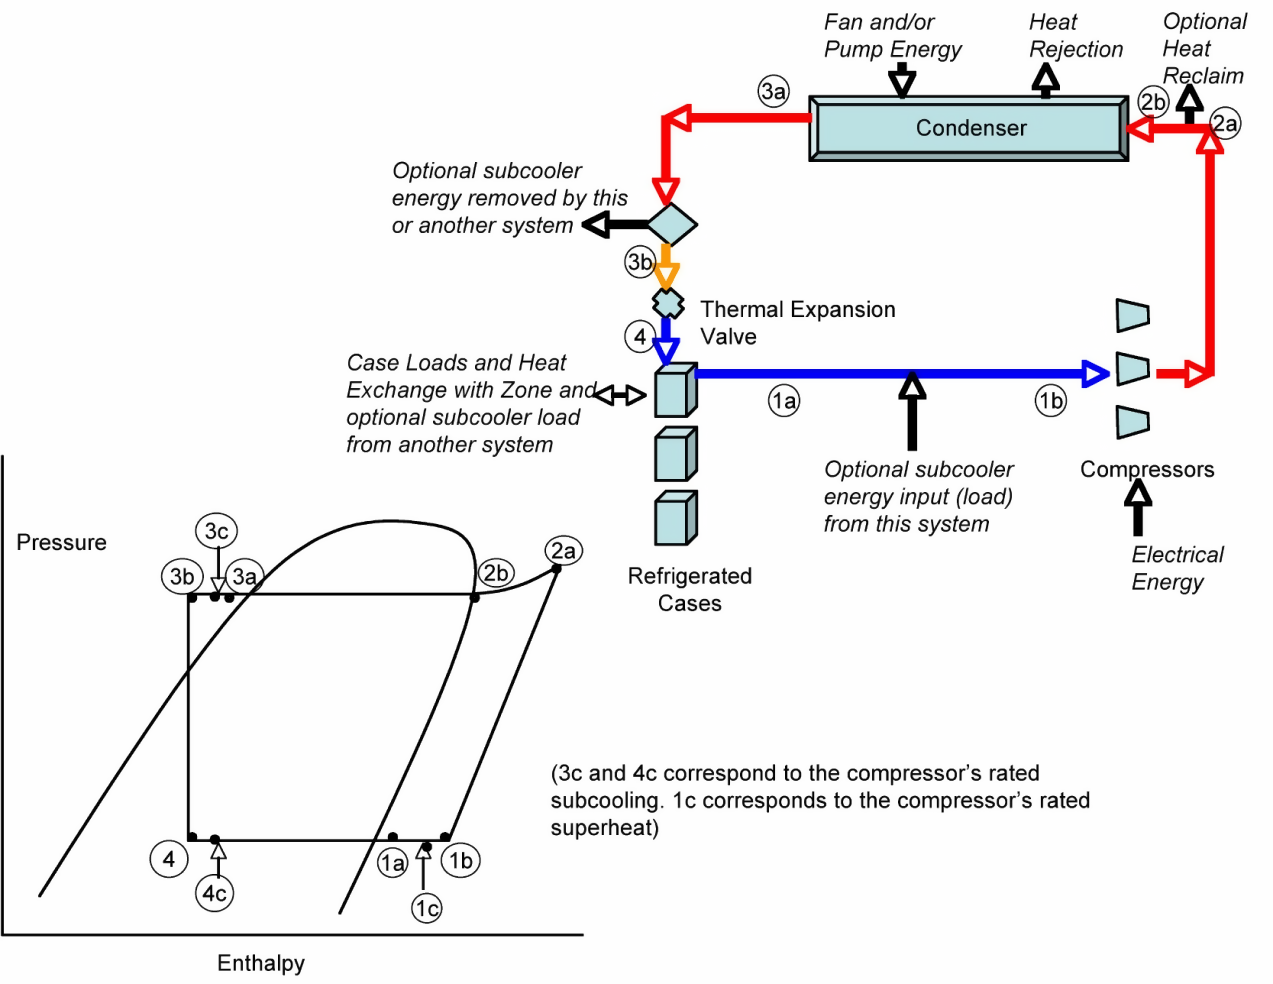
\includegraphics[width=0.9\textwidth, height=0.9\textheight, keepaspectratio=true]{media/image6275.png}
\caption{State Points and Energy Flows for Detailed Refrigeration System \protect \label{fig:state-points-and-energy-flows-for-detailed}}
\end{figure}

Once the corrected capacity is calculated for each compressor, the compressors are dispatched one at a time until the system load is met. The last compressor dispatched is assumed to run at full load for the fraction of the time step necessary to meet the load, That is, the model neglects compressor cycling losses at part-load conditions. Using the state point identification from Figure~\ref{fig:state-points-and-energy-flows-for-detailed}, these corrections are shown in the following equations. If the capacity available from all the compressors is less than the sum of the case loads for that time period, the unmet load is accumulated to be met in succeeding time steps. If this accumulated unmet load becomes too great, a warning message is generated.

\begin{equation}
  \begin{array}{rl}
    Cap_{corrected} &= \frac{\rho_{1b}}{\rho_{1c}} \times \frac{h_{1b} - h_4}{h_{1c} - h_{4c}} Cap_{rated} \\
    \dot{m} &= \frac{Cap_{corrected}}{h_{1b} - h_4}
  \end{array}
\end{equation}

where:

\(\dot m\) is the mass flow rate of refrigerant (kg/s)

\(\rho\) is the density (kg/m\(^{3}\))

h is the enthalpy (J/kg)

Cap is the refrigeration capacity of an individual compressor (W).

Compressor performance can also be improved by allowing the suction pressure to rise whenever the sum of the loads on the refrigerated cases served by the compressors is less than the design load. The calculation of the maximum allowable evaporator temperature is described in ``Variable Evaporator Temperature'' in the discussion of Refrigeration Cases.

\subsubsection{Two-Stage Compression Systems}\label{two-stage-compression-systems}

In addition to the single-stage compression refrigeration system illustrated above, two-stage compression systems can be modeled.~ For low temperature applications where the pressure ratio between the low- and high-pressure sides of the system could be 1:10 or more, it may be beneficial to utilize two stages of compression (Evans 2008).~ Two smaller compressors in series have a smaller displacement and usually operate more efficiently than one large compressor that covers the entire pressure range from the evaporator to the condenser.~ This is especially true in ammonia refrigeration systems due to the large amount of superheating that occurs during the compression process (ASHRAE 2009b).

Between the two stages of compression, an intercooler is used to cool the discharge gas exiting the low-stage compressor before it enters the high-stage compressor.~ The cooling is performed within the intercooler by refrigerant at an intermediate pressure.~ The degree to which intercooling reduces the power requirement of a refrigeration cycle depends on the refrigerant which is being used as well as the temperature lift between the evaporator and the condenser.

Several methods of two-stage compression and intercooling have been used.~ For large industrial refrigeration systems, typical of ammonia systems used in refrigerated warehouses, both shell-and-coil intercooling (Figure~\ref{fig:two-stage-compression-system-with-a-shell}) and flash intercooling (Figure~\ref{fig:two-stage-compression-system-with-a-flash}) are used.~ The two stages of compression in these systems may be performed by separate low- and high-stage compressors or with a compound compressor containing both the low and high stages within the same compressor body.

\begin{figure}[hbtp] % fig 281
\centering
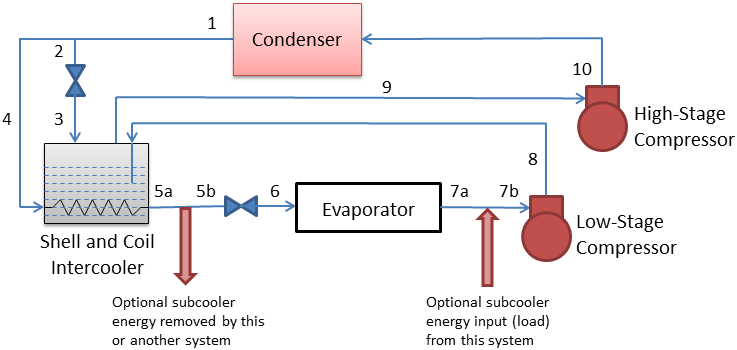
\includegraphics[width=0.9\textwidth, height=0.9\textheight, keepaspectratio=true]{media/image6278.png}
\caption{Two-Stage Compression System with a Shell-and-Coil Intercooler. \protect \label{fig:two-stage-compression-system-with-a-shell}}
\end{figure}

\begin{figure}[hbtp] % fig 282
\centering

\includegraphics[width=0.9\textwidth, height=0.9\textheight, keepaspectratio=true]{media/image6279.png}
\caption{Two-Stage Compression System with a Flash Intercooler. \protect \label{fig:two-stage-compression-system-with-a-flash}}
\end{figure}

For two-stage compression systems with intercooling, there is an optimum intermediate pressure that minimizes the total power consumption of the system.~ In the case of an ideal intercooler in which the refrigerant gas enters the high-stage compressor at the same temperature as it enters the low-stage compressor, the minimum compressor work is achieved using the same pressure ratio across both compressors (Baek et al. 2005).~ Typically, the optimum intermediate pressure is approximated as the geometric mean pressure of the system as follows:

\begin{equation}
{P_{{\mathop{\rm int}} ercooler}} = \sqrt {\left( {{P_{evaporator}}} \right)\left( {{P_{condenser}}} \right)}
\end{equation}

where \emph{P\(_{intercooler}\)} is the pressure within the intercooler shell, \emph{P\(_{evaporator}\)} is the evaporating pressure and \emph{P\(_{condenser}\)} is the condensing pressure.

The low-stage compressors operate between the evaporator pressure and the intercooler pressure while the high-stage compressors operate between the intercooler pressure and the condensing pressure.~ The performance of both the low-stage and high-stage compressors are modeled using the compressors' performance curves defined by ARI Standard 540 (ARI 2004), as discussed previously in the ``Compressor Energy Use'' section.~ In addition, capacity corrections are applied to the compressor performance curves to account for deviations between the actual operating conditions and the rated conditions.

Referring to Figure~\ref{fig:two-stage-compression-system-with-a-shell} for a two-stage system with a shell-and-coil intercooler, the performance of the intercooler is modeled with a ``Shell-and-Coil Intercooler Effectiveness'', defined as follows:

\begin{equation}
\eta  = \frac{{{T_4} - {T_{5a}}}}{{{T_4} - {T_3}}}
\end{equation}

where \(\eta\) is the shell-and-coil intercooler effectiveness, \emph{T}\(_{4}\) is the inlet temperature of the liquid refrigerant at Location 4, \emph{T}\(_{5a}\) is the outlet temperature of the liquid refrigerant at Location 5a, and \emph{T}\(_{3}\) is the saturated refrigerant temperature within the intercooler shell.~ Valid values for the effectiveness range from 0.0 to 1.0.~ An effectiveness of zero indicates that no heat is transferred from the refrigerant in the shell-side of the intercooler to the liquid refrigerant in the coil-side of the the intercooler, and thus, there is no change in the temperature of the liquid refrigerant from Location 4 to Location 5a.~ An effectiveness of 1.0 indicates that the temperature of the liquid exiting the coil-side of the intercooler at Location 5a is equal to the temperature of the saturated refrigerant in the shell-side of the intercooler.~ The user may specify a value for the intercooler effectiveness and a default value of 0.8 is used if no value is specified.~ Furthermore, it is assumed that saturated vapor refrigerant exits the shell-and-coil intercooler at Location 9.

For the flash intercooler shown in Figure~\ref{fig:two-stage-compression-system-with-a-flash}, it is assumed that saturated liquid exits the intercooler at Location 3a and saturated vapor refrigerant exits the intercooler at Location 7.

The two-stage compression refrigeration system may include an optional mechanical subcooler or liquid-suction subcooler.~ These subcoolers cool the liquid refrigerant which exits the intercooler before the refrigerant enters the thermal expansion valve.~ Further details regarding the modeling of mechanical and liquid-suction subcoolers may be found in the ``Subcoolers'' section.

\subsubsection{Condenser Performance}\label{condenser-performance}

Only one condenser is allowed per system. However, multiple refrigeration systems can reject heat through the same condenser. If a single condenser is used by multiple refrigeration systems, the code will iterate just as it does for loads transferred between systems to ensure that the total load on the condenser is accounted for in determining the saturated condensing temperature.

The condenser can be modeled as dry air cooling, wet evaporative cooling, water loop cooling, or cascade cooling. (The detailed system can not be used for a compressor rack discharging heat into a conditioned zone.) The condenser performance is modeled to determine: (1) the condensing temperature and enthalpy of the refrigerant entering the refrigerated cases attached to the suction group, both of which will influence the efficiency of the compressors, (2) auxiliary power consumption for fans and pumps, and (3) water consumption for evaporative and water-cooled condensers.

EnergyPlus can simulate waste heat being reclaimed from a detailed refrigeration system for use by refrigerant-to-air and refrigerant-to-water heating coils. (Refer to objects Coil:Heating:Desuperheater and Coil:WaterHeating:Desuperheater for a complete description of how these coils are modeled.) Heat reclaimed from the detailed refrigeration system is limited to the portion of the rejected heat in the superheat region. Using the state point nomenclature from Figure~\ref{fig:state-points-and-energy-flows-for-detailed}, this value is calculated by the detailed compressor and condenser models each time step as follows:

\begin{equation}
{\dot Q_{AvailableSuperheat}} = \dot m \left( {{h_{2a}} - {h_{2b}}} \right)
\end{equation}

Heat reclaimed for hot gas or hot brine defrost is not limited to the superheat range. However, if an excessive amount of the system rejected heat is diverted for that purpose, a warning is issued advising the user to increase the diversity of the defrost schedules.

The total heat rejection load on the condenser is the sum of the case and walk-in loads, any transfer loads (e.g., mechanical subcooler or secondary system (see object Refrigeration:SecondarySystem)) on the system(s), and the total compressor power. The condenser load is reduced by any heat reclaimed by desuperheating coils for HVAC or water heating purposes and hot gas or hot brine defrost. If a secondary system or cascade condenser is served by the system(s) using this condenser, any defrost heat rejection credits from loads on the secondary system are assigned to this condenser.

\begin{equation}
{\dot Q_{Rejected}} = \sum {{{\dot Q}_{System}}}  - \sum {{{\dot Q}_{Reclaimed}}}
\end{equation}

where:

\(\dot{Q}_{Rejected}\) is the heat rejected by the condenser (W)

\(\sum {{{\dot Q}_{Reclaimed}}}\) is the sum of all the heat reclaimed by desuperheater coils and hot gas and hot brine defrost (W).

Depending upon the condenser type, the heat rejection environment is set to the ambient conditions, conditions corresponding to a defined outside air node (sometimes used to represent condensers located above ground level) or zone node, to a temperature specified for a water-cooled condenser, or according to the evaporating temperature for a higher-temperature loop (used for cascade condensers).

The enthalpy of the condensed refrigerant leaving the condenser is equal to:

\begin{equation}
{h_{condenser,out}} = {h_{sat,liquid}}({T_{condense}}) - {c_{p,sat,liquid}}({T_{condense}}) \cdot \Delta {T_{RatedSubcooling}}
\end{equation}

where:

\(h_{condenser,out}\) is the enthalpy leaving the condenser (J/kg)

\(h_{sat,liquid}\) is the enthalpy of saturated liquid at the condensing temperature (J/kg)

\(c_{p,sat,liquid}\) is the specific heat of saturated liquid at the condensing temperature )J/kg-\(^{\circ}\)C)

\(\Delta T_{RatedSubcooling}\) is the amount of subcooling included in condenser rated heat rejection (\(^{\circ}\)C).

A minimum condensing temperature is specified for the detailed refrigeration system, and is usually required to maintain acceptable thermal expansion valve performance. When the calculated condensing temperature is less than this minimum, the air flow for air and evaporative-cooled condensers is reduced to reduce the condenser capacity and maintain the required condensing temperature.

\paragraph{Air-Cooled Condensers}\label{air-cooled-condensers}

The heat rejection capacity of a dry air-cooled condenser object (Refrigeration:Condenser:AirCooled) is directly proportional to the difference between the condensing temperature and the drybulb temperature for the heat rejection environment. The manufacturers typically provide the performance data, at one standard atmosphere, in a linear relationship between heat rejection and temperature difference. A correction factor is applied to account for the variation in air density with elevation (Carrier 1999).

\begin{equation}
  \begin{array}{rl}
    Hrej_{Rated} &= C_1 + C_2 \PB{T_{condenser} - T_{drybulb}} \\
    Hrej_{Rated,corrected} &= Hrej_{Rated} \PB{1 - \PB{7.17E-5 \times Elevation}}
  \end{array}
\end{equation}

where:

Hrej\(Hrej_{Rated}\) is the manufacturer's rated heat rejected by the condenser (W)

\(C_{1}\) is the intercept taken from manufacturer's condenser performance data (W)

\(C_{2}\) is the coefficient taken from the manufacturer's condenser performance data (W/\(^{\circ}\)C)

\(T_{condense}\) is the condensing temperature (\(^{\circ}\)C)

\(T_{drybulb}\) is the drybulb temperature for the local environment (\(^{\circ}\)C)

Elevation is the local elevation (m)

The manufacturer's form of performance data is used internally to define the condensing temperature as a function of the heat rejection load.

\begin{equation}
{T_{condense}} = {T_{drybulb}} + \left( {\frac{{Hrej - {C_1}}}{{{C_2}}}} \right) \div (1 - 7.17E - 5 \times Elevation)
\end{equation}

This calculated condensing temperature is then compared to the minimum condensing temperature allowed for that system. If necessary, the air flow to the condenser is reduced to maintain the condensing temperature at or above that minimum value.

\paragraph{Condenser Fan Energy Use}\label{condenser-fan-energy-use-1}

Condenser fan power for air-cooled condensers is determined by the type of fan control, fixed, variable speed, or two-speed. For all three fan control types, the fan power is set equal to the rated fan power whenever the calculated condensing temperature is greater than or equal to the minimum allowed condensing temperature. If the calculated temperature is less than the minimum allowed, the condenser air flow must be reduced. The reduced rated capacity is calculated using the previous equation for \emph{Hrej\(_{Rated}\)} with the specified minimum condensing temperature. (Note, the minimum condensing temperature is often determined by the expansion valve performance, and is therefore input with the system description, not with the condenser description.) The air flow for the reduced condenser capacity is:

\begin{equation}
  \begin{array}{rl}
    Hrej &\propto \text{AirVelocity}^N \\
    \text{Air Velocity} &\propto Hrej^{1/N} \\
    \text{Air Volume Ratio} &= \PB{\frac{Hrej}{Hrej_{Rated}}}^{1/N}
  \end{array}
\end{equation}

where N is 0.633 for turbulent air flow over cylinders (ASHRAE 2005).

The Air Volume Ratio is limited by a minimum value, which may be specified by the user. The default for this value is 0.2.

Four fan curves are built into the condenser fan model to represent four types of fan control, as shown in Figure~\ref{fig:condenser-fan-power-curve-options}. (Lawrence Berkeley Laboratory and Resource Dynamics, April 2003)

\begin{figure}[hbtp] % fig 283
\centering
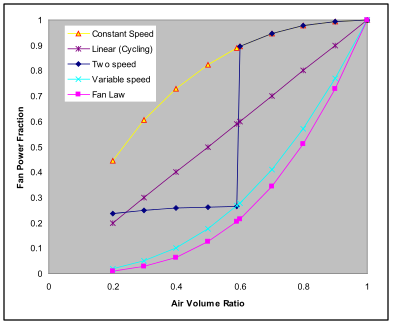
\includegraphics[width=0.9\textwidth, height=0.9\textheight, keepaspectratio=true]{media/image6291.svg.png}
\caption{Condenser fan power curve options \protect \label{fig:condenser-fan-power-curve-options}}
\end{figure}

For a fixed-speed fan, the air flow is reduced through either the use of dampers or by cycling the fan on and off.

For a cycling fan, the power variation with air flow volume is approximately linear above the minimum air volume ratio as shown in the following equation for the option ``FixedLinear'':

\begin{equation}
{P_{CondFan}} = ({\rm{Air~Volume~Ratio}}){P_{CondFan,design}}
\end{equation}

where:

\({P_{CondFan}}\) is the output variable ``Refrigerated Case Condenser Fan Electric Power {[}W{]}'', not allowed to exceed the design condenser fan power

\({P_{CondFan,design}}\) is the design condenser fan power (W).

For a fixed speed fan with damper (corresponding to the option ``Fixed''), the shape of the power fraction curve is as shown above, and calculated using:

\begin{equation}
{P_{CondFan}} = ({Air~Volume~Ratio}){e^{(1 - {Air~Volume~Ratio})}}{P_{CondFan,design}}
\end{equation}

For an ideal variable speed fan, the power is proportional to the cube of the air flow. To reflect non-ideal real systems, an exponent of 2.5 is used as shown in the following equation:

\begin{equation}
{P_{CondFan}} = {({Air~Volume~Ratio})^{2.5}}{P_{CondFan,design}}
\end{equation}

For a two-speed fan, the fan power is varied as for a constant speed fan with dampers for Air Volume Ratios greater than or equal to 0.6. For lower Air Volume Ratios,~ which correspond to a half-speed fan setting, the power is reduced to the variable fan power value at that point and then varied as for damper control below Air Volume Ratios (AVR) of 0.6.

\begin{equation}
  P_{CondFan} = \left\{ \begin{array}{cr}
                          \PB{AVR}\PB{e^{\PB{1-AVR}}}P_{CondFan,Design} & if~AVR \geq 0.6 \\
                          \PB{\frac{AVR+0.4}{2^{2.5}}}\PB{e^{\PB{1-AVR}}}P_{CondFan,Design} & if~AVR < 0.6
                        \end{array}
                \right.
\end{equation}

For a water cooled condenser, there is no fan load at the condenser (i.e., the~ water/refrigerant heat exchanger). Any fan load would be related to and accounted for at the heat rejection object (e.g., cooling tower)

\paragraph{Evaporative-Cooled Condensers}\label{evaporative-cooled-condensers}

The input object Refrigeration:Condenser:EvaporativeCooled allows using evaporative cooling rather than dry air cooling which will allow for more efficient condenser heat rejection based on the entering air approaching the wet-bulb temperature rather than the dry-bulb temperature. Analyses under the International Energy Agency's (IEA) Heat Pumping Programme Annex 26 indicates that this measure can improve refrigeration system efficiency by up to 10\% (IEA 2003). The basin heater energy and water pumping power consumption for evaporative condensers in the detailed refrigeration system is modeled as described for the Refrigeration:CompressorRack. Just as for air-dried condensers, an elevation correction is needed to adjust for the variation in density of the air. This correction factor was derived by combining the barometric pressure correction from ARI 490 and a standard correlation for barometric pressure as a function of elevation(ARI 2008, NASA 1976).

\begin{equation}
  \begin{array}{rl}
    Hrej_{Rated,Corrected} &= Hrej_{Rated} \RB{ 1 + k_1 B P_{std} \PB{1 - e^{\PB{A \times Elev}}}} \\
    A &= \frac{g_0 M_0}{R* T_b} = - 0.00012m^{-1}
  \end{array}
\end{equation}

where

k\(_{1}\) is 0.0023 for pressure stated in kPa, (ARI 2008)

BP\(_{std}\) is the standard atmosphere at rating conditions (101.0 kPa)

g\(_{0}\) is the gravitational constant (9.80665 m/s\(^{2}\))

R* is the universal gas constant (8.31432E3 N-m/kmol-K)

M\(_{0}\) is the molar mass of air (28.9644 kg/kmol)

T\(_{b}\) is the standard temperature (288.15 K).

Although based upon an exponential relationship, the resulting correction is very nearly linear within the range of elevations found upon dry land, so the following form of correction is used:

\begin{equation}
Hre{j_{Rated,Corrected}} = Hre{j_{Rated}} \times (1 - 3.07E - 5 \times Elevation)
\end{equation}

To calculate the condensing temperature for an evaporative cooled condenser, it is necessary to provide the manufacturer's performance data. The manufacturers typically provide this data as a table of condensing temperature as a function of both entering wet-bulb temperature and the ratio of the heat rejected to the rated heat rejected. This data can be well represented, as shown in Figure~\ref{fig:comparison-of-the-condensing-temperature}, by a regression of the form:

\begin{equation}
\PB{T_{condense} - T_{wetbulb}} = {C_1} + {C_2}{HRCF} + \frac{C_3}{HRCF} + {C_4}{T_{wetbulb}}
\end{equation}

or:

\begin{equation}
T_{condense} = {C_1} + {C_2}{HRCF} + \frac{C_3}{HRCF} + \PB{1 + C_4}T_{wetbulb}
\label{eq:TcondenseHRCFTwetbulb}
\end{equation}

Where:

\begin{equation}
HRCF = \frac{Hrej_{Rated}}{Hrej}
\end{equation}


C\(_{1}\), C\(_{2}\), C\(_{3}\), and C\(_{4}\) are coefficients determined by regression from manufacturer's data.

Figure~\ref{fig:comparison-of-the-condensing-temperature} shows a comparison between this equation form, which produced an adjusted R\(^{2}\) of 0.998 and a maximum residual of 0.7\(^{\circ}\)C, for one manufacturer of evaporative condensers. Data from two other manufacturers showed similar agreement with this parameterization.

\begin{figure}[hbtp] % fig 284
\centering
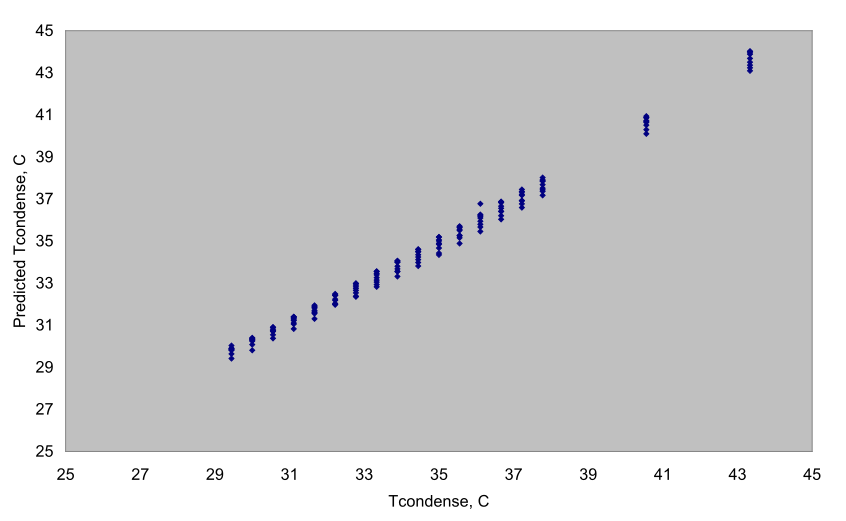
\includegraphics[width=0.9\textwidth, height=0.9\textheight, keepaspectratio=true]{media/image6301.svg.png}
\caption{Comparison of the condensing temperature predicted by four-factor equation to manufacturer's data \protect \label{fig:comparison-of-the-condensing-temperature}}
\end{figure}

Again, the condensing temperature is not allowed to fall below the system's minimum allowed condensing temperature. Just as with an air-cooled condenser, the air flow through the condenser is controlled to maintain this minimum condensing temperature and the air velocity reduction is a function of the decreased capacity (Manske, 1999). For an evaporative condenser, relevant capacity is not the amount of heat rejected, but the rated capacity at that reduced air flow. That decreased rated capacity must first be calculated based upon the specified minimum condensing temperature. Using Equation~\ref{eq:TcondenseHRCFTwetbulb}, the specified condensing temperature is used to calculate the reduced HRCF, which is used with the current heat rejection to calculate the ``reduced Rated Heat Rejection''.

\begin{equation}
0 = C_2 \times HRCF^2 + \left( \RB{C_1 + C_4 T_{wetbulb} - \left( \PB{T_{condenser} - T_{wetbulb}}}\right) \right) \times HRCF + C_3
\end{equation}

\begin{equation}
{Reduced~Rated~Heat~Rejection} = HRCF \times Hrej
\end{equation}

\begin{equation}
{Air~Volume~Ratio} = \PB{\frac{Reduced~Rated~Heat~Rejection}{Hrej_{Rated}}}^{1/N}
\end{equation}

where N = exponent for evaporative condensers, set to 0.76 (Manske, 1999).

The water consumption for an evaporative condenser is calculated based upon the air flow rate, the total heat rejection, and the heat rejection environment. The amount of water consumption also includes the amount of water that is purged to reduce the concentration of contaminants. The purge water is estimated as proportional to the heat rejection, at a rate of 5.0E-10 m\(^{3}\)/s per Watt of heat rejection (B.A.C., 2007). (This value, which corresponds to 3 gal./min. per 100 tons, is slightly more conservative than the value quoted by ASHRAE, 2004.) For the compressor racks, the condenser effectiveness was input as a function of the environmental wetbulb temperature. For the detailed evaporative condenser, the input data instead describes the capacity as a function of environmental conditions and loading. From that data, the water evaporation is calculated using the effectiveness corresponding to a fully loaded condenser. When the condenser is operating outside the bounds of the manufacturer's data, the effectiveness is limited to a maximum value of 0.9.

\begin{equation}
  \begin{array}{rl}
    \eta &= \frac{Hrej}{\dot{V}_{air,rated} \rho_{air} \PB{h_{Tcondense,sat} - h_{air,in}}} \\
    h_{air,out} &= h_{air,in} + \eta \PB{h_{Tcondense,sat} - h_{air,in}} \\
    T_{air,out} &= T_{saturated}\PB{h_{air,out},P_{barometric}} \\
    \dot{V}_{evaporation} &= \frac{{AirVolumeRatio} \cdot \dot{V}_{air,rated} \cdot \rho_{air,dry} \cdot \PB{\omega_{air,out} - \omega_{air,in}}}{\rho_{water}} \\
    \dot{V}_{makeup} &= \dot{V}_{evaporation} + \dot{V}_{purge}
  \end{array}
\end{equation}

where:

\({h_{Tcondense,sat}}\) is the enthalpy of saturated air at the calculated condensing temperature

\(h_{air,out}\) is the enthalpy of the air leaving the condenser

\(h_{air,in}\) is the enthalpy of the inlet air, psychometric function of inlet air drybulb temperature and humidity ratio

\({\dot V_{air,rated}}\) is the rated volumetric air flow for the evaporative condenser (input value) m\(^{3}\)/s

\(\rho_{air}\) is the density of air evaluated at environmental conditions

\(\rho_{air,dry}\) is the density of dry air evaluated at environmental temperature

\(T_{air,out}\) is the air temperature leaving the condenser, psychometric function of saturated air at the enthalpy leaving the condenser and the barometric pressure

\({\dot V_{evaporation}}\) is the volumetric rate of water evaporation in the condenser (m\(^{3}\)/s)

\(\omega_{air,out}\) is the humidity ratio (kg\(_{water}\)/kg\(_{dry~air}\)) of the air leaving the condenser, psychometric function of T\(_{air,out}\) and the barometric pressure

\(\omega_{air,in}\) is the humidity ratio (kg\(_{water}\)/kg\(_{dry~air}\)) of the air at environmental conditions

\(\rho_{water}\) is the density of water evaluated at the environmental wetbulb temperature (kg/m\(^{3}\))

\({\dot V_{purge}}\) is the volumetric rate of water purged in the condenser (m\(^{3}\)/s)

\({\dot V_{makeup}}\) is the volumetric rate of water makeup in the condenser (m\(^{3}\)/s).

The source of the makeup water may be specified as a water storage tank. If not specified, the makeup water is assumed to come from the building mains (Ref. Water Mains Temperatures).

An evaporative condenser can be scheduled, using the Evaporative Condenser Availability Schedule described previously, so that it operates in a dry mode for a portion of the year. This is important in climates subject to freezing weather in order to avoid excessive ice formation on the condenser surfaces and surroundings. (The Availability Schedule is the correct way to model the use of evaporative condensers in cold climates. However, some users may take a single input description and use it to model a building with a refrigeration system in a variety of climates. To avoid modeling the use of evaporative coolers in freezing weather, the code includes a cutout to switch to dry operation whenever the outdoor drybulb temperature drops below 4\(^{\circ}\)C.) Dry operation can also reduce water use when the dry heat rejection capacity of the equipment is sufficient to meet the load during times of the year when the outside drybulb temperature is reduced. In dry operation, the condenser heat rejection capacity is approximately one third of the rated wetted heat rejection capacity(Manske, 2000). In dry operation, the condensing temperature is estimated by using the same four-factor equation, but using the air drybulb temperature instead of the wetbulb temperature and using the reduced heat rejection capacity factor.

\begin{equation}
  \begin{array}{rl}
    HRCF_{dry operation} &= \frac{HRCF_{wet operation}}{3.0} \\
    T_{condense,dry operation} &= {C_1} + {C_2}{HRCF_{dry operation}} + \frac{C_3}{HRCF_{dry operation}} + \PB{1 + C_4} T_{drybulb}
  \end{array}
\end{equation}

\paragraph{Water-Cooled Condensers}\label{water-cooled-condensers}

If the condenser heat rejection is specified as water cooled (input object Refrigeration:Condenser:WaterCooled), the model uses the same algorithms described above for Refrigeration Compressor Racks. The condensing temperature is set equal to the inlet water temperature plus an approach temperature equal to the difference between the rated values for water inlet temperature and condensing temperature.

\paragraph{Cascade Condensers}\label{cascade-condensers}

A cascade condenser joins two full detailed refrigeration systems; that is, both systems joined by the cascade condenser have loads, compressor(s), and a condenser, as shown in Figure~\ref{fig:a-cascade-condenser-is-used-to-reject-heat}.

\begin{figure}[hbtp] % fig 285
\centering
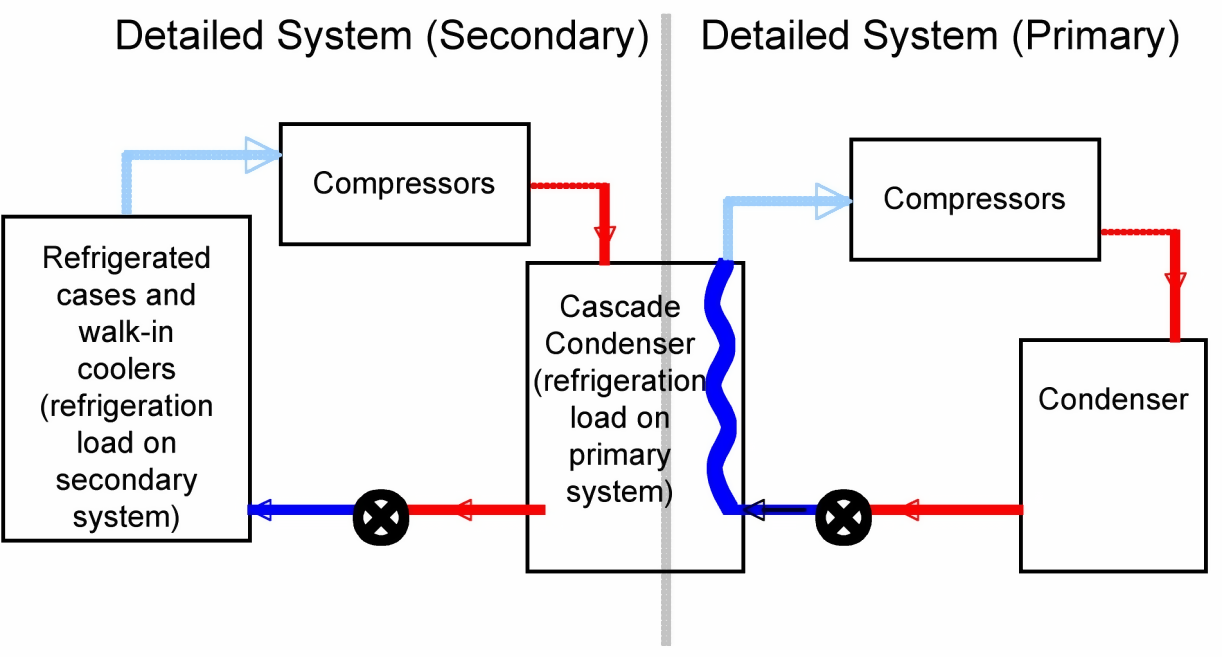
\includegraphics[width=0.9\textwidth, height=0.9\textheight, keepaspectratio=true]{media/image6310.png}
\caption{A cascade condenser is used to reject heat from a low-temperature detailed refrigeration system to a higher-temperature detailed refrigeration system \protect \label{fig:a-cascade-condenser-is-used-to-reject-heat}}
\end{figure}

The input object, Refrigeration:Condenser:Cascade, allows the use of a higher temperature refrigeration system (primary system) to serve as a heat rejection sink for a lower temperature refrigeration system (secondary system). The selection of the condensing temperature represents a trade-off in performance between the primary system absorbing the heat rejection and the secondary system rejecting heat. (Lee et al., 2006) If the condensing temperature control type is `fixed,' then the secondary system condensing temperature is held constant at the temperature specified for that cascade condenser (which should be greater than or equal to the secondary system's specified minimum condensing temperature). If the condensing temperature control type is `float', the condensing temperature is allowed to float according to the minimum required evaporating temperature for other loads served by the primary system.

For fixed control:

\begin{equation}
T_{condense} = T_{condense,rated}
\end{equation}

For floating control:

\begin{equation}
T_{condense} = \Delta{T_{approach}} + T_{evap,min}
\end{equation}

where:

T\(_{condense,rated}\) is the rated condensing temperature for the cascade condenser (\(^{\circ}\)C)

ΔT\(_{approach}\) is the rated approach temperature difference for the cascade condenser (\(\Delta^{\circ}\)C)

T\(_{evap,min}\) is the evaporating temperature required to meet other loads on the primary system (\(^{\circ}\)C).

The approach temperature difference (the difference between the condensing and evaporating temperatures) in the cascade condenser, is held constant at the rated value.~ That is, the approach temperature difference is not varied according to the load on the condenser.

For cases and walk-ins served by cascade condensers, energy needed for hot brine or hot gas defrost is reclaimed from the primary system.~ The refrigeration load the cascade condenser places upon the primary system is classified as a `transfer load', because it transfers load from one system to another. This load is the sum of all case and walk-in loads served by the secondary system, any suction piping heat gains on the secondary loop, plus the secondary loop's compressor power. The same name (Ref. Refrigeration:Condenser:Cascade, field ``Name'') used to identify the condenser in the secondary loop is used to identify the transfer load on the primary system.

\begin{equation}
{\dot Q_{{\rm{Cascade}}}} = {\sum {\dot Q}_{{\rm{Case}}}} + \sum {{{\dot Q}_{{\rm{Walkin}}}} + } \sum {{{\dot Q}_{{\rm{Compressor}}}}} \left( { + \sum {{{\dot Q}_{{\rm{PipeHeatGain}}}}} } \right)
\end{equation}

where:

\({\dot Q_{Cascade}}\) is the total refrigeration load the cascade condenser places upon the primary system (W)

\({\dot Q_{Case}}\) is the case load on the secondary loop (W)

\({\dot Q_{Walkin}}\) is the walk-in load on the secondary loop (W)

\({\dot Q_{Compressor}}\) is the power input to a compressor on the secondary loop (W)

\({\dot Q_{PipeHeatGain}}\) is the heat gain in secondary loop suction pipe (W).

\textbf{Even though a cascade condenser is considered to be a part of a secondary loop, that loop is described with the Refrigeration:System object, not with the object, Refrigeration:SecondarySystem, described below.}

\subsubsection{Subcoolers}\label{subcoolers}

Subcooler objects (Refrigeration:Subcooler) reduce the temperature of the liquid refrigerant after it leaves the condenser and before it reaches the thermal expansion valve, corresponding to state point, 3b, on Figure~\ref{fig:state-points-and-energy-flows-for-detailed}. The detailed refrigeration system permits the use of two type of subcoolers, mechanical and liquid suction. A mechanical subcooler is used to transfer refrigeration load from a lower-temperature system to a higher-temperature system. For example, the compressors that are used to provide cooling for dairy products could be used to subcool the refrigerant in another system that is serving frozen food cases. For the system providing the cooling, the mechanical subcooler acts like another refrigerated case load. For the system receiving the cooling, the mechanical subcooler reduces the enthalpy of the refrigerant from point 3a to point 3b on Figure~\ref{fig:state-points-and-energy-flows-for-detailed}, and thus reduces the required refrigerant flow rate. Mechanical subcooler performance is defined by the controlled temperature of the subcooled liquid as follows:

\begin{equation}
  \begin{array}{rl}
    \dot{Q} &= \dot{m} C_p \PB{T_{3a} - T_{control}} \\
    h_{3b}  &= h_{3a} - C_{p,liquid} \PB{T_{3a} - T_{control}}
  \end{array}
\end{equation}

where:

\(\dot Q\) is the subcooler load (W)

\(\dot m\) is the mass flow rate of refrigerant (kg/s)

\(c_{p,liquid}\) is the specific heat of saturated liquid at the condensing temperature, (J/kg-\(^{\circ}\)C)

\(T_{control}\) is the control temperature specified for the mechanical subcooler (\(^{\circ}\)C)

\emph{h} is the enthalpy (J/kg).

A liquid suction heat exchanger (LSHX) subcooler uses the cold gas exiting the refrigerated cases to subcool the condensed liquid refrigerant in the same system. Depending upon the shape of the refrigerant's saturation curve and the operating condensing and evaporating temperature, this can save significant energy by reducing the required refrigerant flow (ASHRAE 2006a). (This model neglects the pressure drop through the suction side of the heat exchanger, although this pressure drop will cause the compressor to operate at a lower suction pressure.) A liquid suction heat exchanger is defined by specifying the design values for: inlet liquid temperature, inlet vapor temperature, and liquid temperature change. A liquid suction heat exchanger subcooler will also increase the superheat of the gas returning to the compressor, as shown by the difference between state points 1a and 1b in Figure~\ref{fig:state-points-and-energy-flows-for-detailed}:

\begin{equation}
  \begin{array}{rl}
    \eta_{LSHX} &= \frac{\Delta T_{Design}}{T_{Liquid Design} - T_{Vapor Design}} \\
    \dot{Q} &= \dot{m} C_{p,liquid} \eta_{LSHX} \PB{T_{3a} - T_{1a}} \\
    T_{1b} &= T_{1a} + \frac{\dot{Q}}{\dot{m}C_{p,vapor}} \\
    h_{3b} &= h_{3a} - \frac{\dot{Q}}{\dot{m}}
  \end{array}
\end{equation}

where:

\({\eta_{LSHX}}\) is the subcooler effectiveness

\(c_{p,vapor}\) is the specific heat of saturated vapor at the evaporating temperature (J/kg-\(^{\circ}\)C)

\(\Delta T_{Design}\) is the design liquid temperature difference (\(\Delta^{\circ}\)C)

\(T_{LiquidDesign}\) is the design liquid inlet temperature (\(^{\circ}\)C)

\(T_{VaporDesign}\) is the design vapor inlet temperature (\(^{\circ}\)C).

If a system is subcooled by both a mechanical subcooler and a liquid subcooler, the liquid subcooler will follow the mechanical subcooler and those points labeled `3a' in the liquid suction equations would correspond to the points labeled `3b' in the mechanical subcooler equations, that is, the inlet of the LSHX would be the outlet of the mechanical subcooler.

Any one system can be cooled (i.e., have energy removed between points `3a' and `3b') by at most one liquid suction heat exchanger and one mechanical subcooler. However, a system can provide cooling to multiple mechanical subcoolers. For example if a building had one high temperature refrigeration system (perhaps cooling fresh produce) and three low temperature systems (perhaps cooling frozen foods and meat), each of the three low temperature systems could include a mechanical subcooler with the refrigeration energy for all three absorbed by the one high-temperature system. For the compressors and condenser on the high-temperature system, these three mechanical subcoolers would represent a load very similar to that of the refrigerated cases served by that system.

\subsubsection{Suction Piping Heat Gains}\label{suction-piping-heat-gains}

Suction piping heat gain is an optional element in the load calculation.~ Typically, the suction pipe heat gain is small compared to the other loads.~ However, when comparing DX systems to secondary systems, this portion of the total load can be very different. (Hinde, D., et al. 2009) ~To include the suction pipe heat gain load, the user must first calculate the U-value and outer surface area for the suction piping. The U-value is the total conductance from the inside skin coefficient, through the pipe insulation, to the outside skin coefficient. This value must be multiplied by the external surface area of the pipe insulation to provide the sum of the UA required in the input.~ These piping heat gains are also reflected in the zone heat balance.

\begin{equation}
{\dot Q_{PipeHeatGain}} = \sum U A (T_{zone} - T_{SaturatedSuction})
\end{equation}

where:

\({\dot Q_{PipeHeatGain}}\)  is the heat load on the detailed refrigeration system due to suction pipe heat gains (W)

\(\sum U A\)  is the sum of the product of the conductance times the surface area for the suction piping (W/\(^{\circ}\)C).

\subsection{Secondary Refrigeration Systems}\label{secondary-refrigeration-systems}

The object, Refrigeration:SecondarySystem, is used to model systems that do not have compressors, but have a circulating pump and a heat exchanger (called the secondary evaporator) where evaporating refrigerant in the primary loop absorbs heat rejected by the secondary loop.~ The purpose of the secondary refrigeration system model is to determine: the refrigerating load placed upon the primary system via the Secondary Evaporator, the required evaporating temperature in the Secondary Evaporator, any heat recovered for defrost purposes, and the total pump power.

If your secondary loop includes compressors and a cascade condenser, do NOT use a Refrigeration:SecondarySystem object.~ Use a Refrigeration:System object with a Refrigeration:Condenser:Cascade object and list that condenser as a transfer load in the input description of the primary system.

In the secondary loop shown in Figure~\ref{fig:secondary-loop-with-brine-or-glycol-solution}, the secondary evaporator serves to chill a brine or glycol solution (single phase) that in turn chills the refrigeration loads on the secondary loop.~ In Figure~\ref{fig:secondary-loop-with-liquid-overfeed}, the secondary evaporator serves as a condenser for a refrigerant that has been partially vaporized(two-phase) while circulating through the refrigeration loads on the secondary loop. Every secondary system includes a refrigeration load made up of refrigerated cases and/or walkins, a heat exchanger (called the Secondary Evaporator), and circulating pump(s). The loop performance at any one time step is determined by the effectiveness of the heat exchanger, the refrigeration load, and the pumping power needed to meet that load. The fluid temperature entering the cases and walk-ins is maintained at a set value.

\begin{figure}[hbtp] % fig 286
\centering
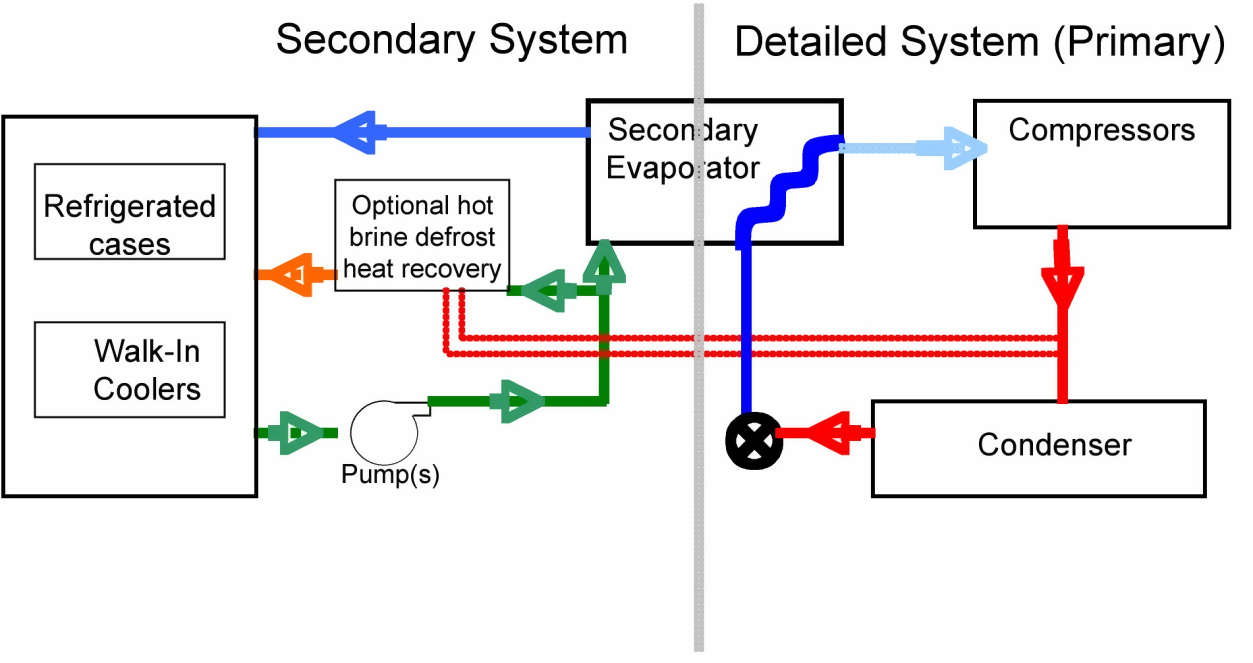
\includegraphics[width=0.9\textwidth, height=0.9\textheight, keepaspectratio=true]{media/image6323.png}
\caption{Secondary loop with brine or glycol solution circulation \protect \label{fig:secondary-loop-with-brine-or-glycol-solution}}
\end{figure}

\begin{figure}[hbtp] % fig 287
\centering

\includegraphics[width=0.9\textwidth, height=0.9\textheight, keepaspectratio=true]{media/image6324.png}
\caption{Secondary loop with liquid-overfeed refrigerant circulation \protect \label{fig:secondary-loop-with-liquid-overfeed}}
\end{figure}

For both types of secondary loops, the primary refrigeration system absorbs the load by providing cold refrigerant that evaporates in the secondary evaporator.~ We classify this secondary load as a `transfer load' because it transfers load from one `system' to another. (Cascade condenser loads are also considered transfer loads.) Just as with any DX refrigeration evaporator, the variable load from the secondary system is served by varying the primary system refrigerant flow to the evaporator side of the secondary evaporator.~ Unmet load will be carried over to the next time step anytime the load on the secondary condenser/evaporator exceeds the rated capacity for the specified temperatures.~ (A warning will be generated if the total unmet energy grows excessively large.) ~The main differences between the single-phase secondary loop model and the two-phase secondary loop model lie in the definition and performance of the secondary evaporator and the way input data is processed to define evaporator capacity.

For a brine system, the secondary loop capacity is matched to the case and walk-in load by varying the brine flow rate. (\emph{Throughout this section, `brine' will be used when referring to the secondary loop heat transfer fluid for systems where the secondary circulating fluid remains in the liquid state.)} When selecting the brine loop design parameters, it is important to consider the performance trade-off between pumping energy and the temperature difference, or range, in the heat exchanger. The circulating fluid selection is also critical in determining the performance of brine loop, with large variations caused by differences in viscosity and density (which impact pumping power requirements) and specific heat (which determines the required fluid flow rate). ~(Kazachki, G. S., and Hinde, D. K., 2006, Faramarzi, R. T., and Walker, D. H. 2004, ASHRAE. 2006c)

For a secondary loop to accommodate a two-phase secondary coolant, additional hardware is required and the system control mode changes. A separator/receiver is required to separate the wet mixture of liquid and gas returning from the refrigeration load, as shown in Figure~\ref{fig:secondary-loop-with-liquid-overfeed}. ~(In the following discussion, we will refer to the secondary fluid in a liquid-overfeed system as CO\(_{2}\).) In Figure~\ref{fig:thermodynamic-cycle-for-a-liquid-overfeed}, which focuses in on the secondary loop alone, the gaseous CO\(_{2}\) moves via thermosiphon effect to the secondary evaporator, where heat is absorbed by the primary system to condense the CO\(_{2}\), which then returns via gravity flow to the separator/receiver.~ The liquid CO\(_{2}\) is pulled from the bottom of the separator/receiver and pumped to the load. The term `liquid overfeed ratio' refers to the ratio of the total pumped mass flow rate (at the point labeled ``1'' on Figure~\ref{fig:thermodynamic-cycle-for-a-liquid-overfeed}) of CO\(_{2}\) to the mass rate of CO\(_{2}\) evaporated at the load (vapor portion of the flow at the point labeled ``5'' on Figure~\ref{fig:thermodynamic-cycle-for-a-liquid-overfeed}). With a variable flow rate(obtained with either a variable-speed pump or multiple constant-speed pumps), the liquid overfeed ratio is maintained at or above the specified value. With a constant flow rate (obtained by specifying a single constant-speed pump), the liquid overfeed ratio will vary to match the capacity of the variable refrigeration load.(Hinde et al 2009) Even though a greater amount of CO\(_{2}\) is circulated than is evaporated, the pumping power requirements are still much less than those for a single-phase secondary coolant.

\begin{figure}[hbtp] % fig 288
\centering
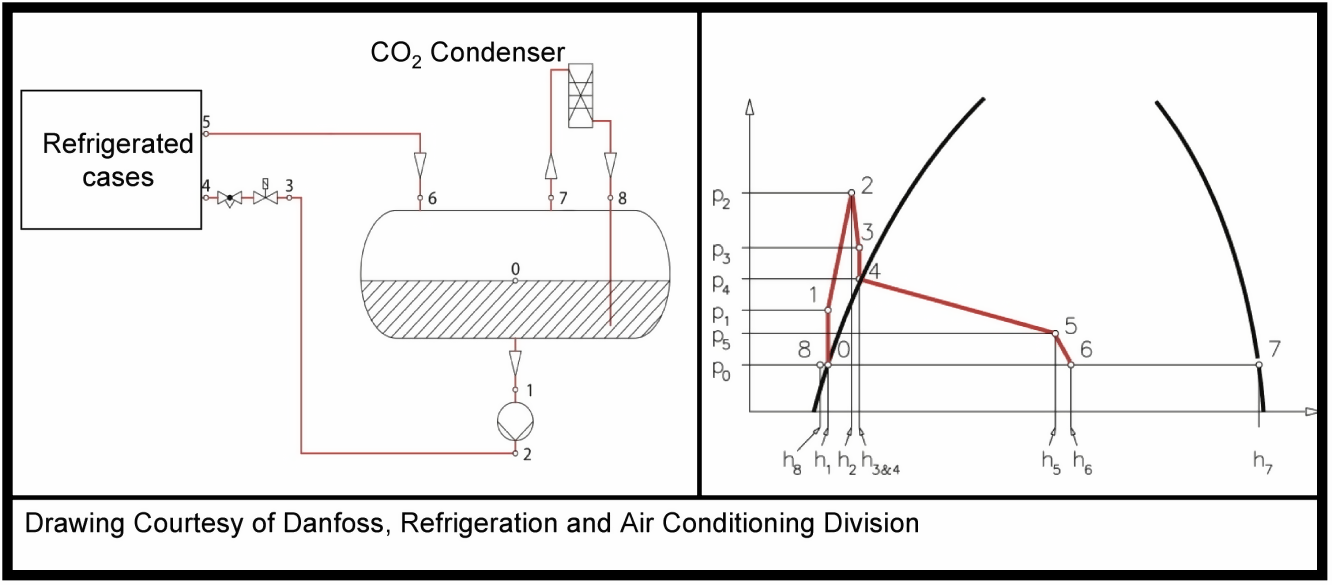
\includegraphics[width=0.9\textwidth, height=0.9\textheight, keepaspectratio=true]{media/image6325.png}
\caption{Thermodynamic cycle for a liquid overfeed secondary loop \protect \label{fig:thermodynamic-cycle-for-a-liquid-overfeed}}
\end{figure}

If the defrost type for any of the cases or walkins on the secondary loop is `HotBrine' or `HotGas', the defrost energy is assumed to come from the hot compressed gas leaving the compressors on the primary system, as shown in Figure~\ref{fig:secondary-loop-with-brine-or-glycol-solution} and Figure~\ref{fig:secondary-loop-with-liquid-overfeed}.(Minea, V. 2007) Therefore, the amount of heat rejected by the condenser for that primary system is reduced by the amount needed for defrost. Some research has shown that the defrost times for cases and walk-ins defrosted using hot brine can be significantly shorter than defrost times for electric or hot gas.(Terrell, W. J. Jr., 1999) The user should consider this factor when describing the input data for cases and walk-ins served by a secondary loop.

\subsubsection{Secondary Evaporator in a Single-Phase Secondary Loop (Brine or Glycol Loop)}\label{secondary-evaporator-in-a-single-phase-secondary-loop-brine-or-glycol-loop}

For a single-phase secondary system, the heat exchanger effectiveness is calculated based upon the input rating data, which includes the evaporating temperature, approach and range temperature differences, and heat exchanger capacity. The rated capacity for the heat exchanger can be specified by either providing the capacity in Watts, or the rated mass flow rate. The density and specific heat both correspond to those properties at the average temperature of the heat exchange fluid within the secondary loop heat exchanger.

These variables are specified by the chiller manufacturer at rated conditions:

\(\Delta T_{Approach}\) is the approach temperature difference (\(\Delta^{\circ}\)C)

\(\Delta T_{Range}\) is the range temperature difference (\(\Delta^{\circ}\)C)

\(T_{EvapDesign}\) is the heat exchanger evaporating temperature (\(^{\circ}\)C)

\(Flow_{RatedVolume}\) is the brine flow rate through the heat exchanger (kg/s)

\(Capacity_{Rated}\) is the heat exchanger cooling capacity (W).

The rated conditions are used to calculate:

\begin{equation}
T_{BrineOutRated} = T_{EvapDesign} + \Delta T_{Approach}
\end{equation}

\begin{equation}
T_{BrineInRated} = T_{BrineOutRated} + \Delta T_{Range}
\end{equation}

\begin{equation}
\eta = Capacity_{Rated} / (Flow_{RatedMass} * C_{pBrine} * (T_{BrineInRated} - T_{EvapDesign}))
\end{equation}

\begin{equation}
T_{BrineAverage} = (T_{BrineOutRated} + T_{BrineInRated})/2
\end{equation}

If the capacity is specified and the flow rate is not, then the flow rate is calculated as:

\begin{equation}
Flow_{RatedMass} = Capacity_{Rated}/(C_{pBrine} * \Delta T_{Range})
\end{equation}

\begin{equation}
Flow_{RatedVol} = Flow_{RatedMass} / {\rho}_{Brine}
\end{equation}

If the flow rate is specified and the capacity is not, the capacity is calculated as:

\begin{equation}
Flow_{RatedMass} = Flow_{RatedVol}*{\rho}_{Brine}
\end{equation}

\begin{equation}
Capacity_{Rated} = Flow_{RatedMass} * C_{pBrine} * \Delta T_{Range}
\end{equation}

Where:

\(\eta\) is the heat exchanger effectiveness (dimensionless and less than one)

\(T_{BrineInRated\\}\) is the heat exchanger brine inlet temperature at rated conditions (\(^{\circ}\)C)

\(T_{BrineOutRated}\) is the heat exchanger brine outlet temperature at rated conditions (\(^{\circ}\)C)

\(T_{BrineAverage}\) is the average brine temperature in the heat exchanger (\(^{\circ}\)C)

\(Flow_{RatedMass}\) is the brine flow rate through the heat exchanger (kg/s)

\(Flow_{RatedVol}\) is the brine flow rate through the heat exchanger (m\(^{3}\)/s)

\(C_{pBrine}\) is the brine specific heat (J/kg-\(^{\circ}\)C)

\(\rho_{Brine}\) is the brine density (kg/m\(^{3}\)).

After the heat exchanger effectiveness has been calculated, the value for the heat exchanger design brine flow rate is compared to the design flow rate for the secondary loop pump(s).~ The maximum flow rate in the loop is limited to the smaller of these two values. The heat transfer capacity corresponding to this maximum flow rate is then calculated and compared to the rated heat exchanger capacity. The maximum load on the heat exchanger is limited to the lesser of these two values, the rated heat exchanger capacity or the capacity corresponding to the maximum loop flow rate.

\begin{equation}
Flow_{MaxVol} = Minimum(Flow_{RatedVol}, Flow_{RatedPumpVol})
\end{equation}

\begin{equation}
Capacity_{AtMaxVolFlow} = Flow_{MaxVol} * \eta *( C_{pBrine} * Density_{Brine})*( T_{BrineInRated} - T_{EvapDesign})
\end{equation}

\begin{equation}
Capacity_{Max} = Minimum(Capacity_{Rated}, Capacity_{AtMaxVolFlow})
\end{equation}

where:

\(Flow_{MaxVol}\) is the maximum loop volume flow, limited by either the pump rating or the heat exchanger rating (m\(^{3}\)/s)

\(Capacity_{AtMaxVolFlow}\) is the secondary loop capacity corresponding to the maximum loop flow rate (W)

\(Capacity_{Max}\) is the maximum secondary evaporator capacity (W).

\subsubsection{Secondary Evaporator in a Two-Phase Secondary Loop~ (Liquid-Overfeed Loop, e.g., CO\(_{2}\))}\label{secondary-evaporator-in-a-two-phase-secondary-loop-liquid-overfeed-loop-e.g.-coux5f2}

For a two-phase system, the secondary evaporator effectiveness is not calculated. Both the evaporating and condensing sides of the heat exchanger are assumed to operate at fixed temperatures.~ If the capacity of the secondary evaporator is not input, it will be calculated as the sum of the rated loads plus the rated pump power.

\begin{equation}
  \begin{array}{rl}
    Capacity_{Rated} &= \text{Input~~~~or:} \\
    Capacity_{Rated} &= \sum \dot{Q}_{Case} + \sum \dot{Q}_{WalkIn} + Power_{Pump} \\
    Capacity_{Max}   &= Capacity_{Rated}
  \end{array}
\end{equation}

If the flow rate through the evaporator is not input, it will be calculated based upon the input value for the Circulating Rate.

\begin{equation}
Flo{w_{{\rm{RatedVol}}}} = \frac{{\sum {{{\dot Q}_{{\rm{Case}}}} + \sum {{{\dot Q}_{{\rm{WalkIn}}}} + Powe{r_{{\rm{Pump}}}}} } }}{{{\rho_{Liquid}}\Delta {h_{fg}}}}
\end{equation}

Where:

\(\rho_{Liquid}\) is the liquid density (kg/m\(^{3}\))

\(\Delta h_{fg}\) is the heat of vaporization (J/kg).

\subsubsection{Secondary Loop Distribution Piping and Receiver Shell Heat Gains}\label{secondary-loop-distribution-piping-and-receiver-shell-heat-gains}

Distribution piping and receiver shell heat gains are optional elements in the load calculation.~ Typically, the distribution pipe and receiver shell heat gains are small compared to the other loads.~ However, when comparing direct expansion systems to secondary systems, this portion of the total load can be very different. (Hinde, D., et al. 2009) To calculate the pipe heat gain load, the user must first calculate the U-value and area for the distribution piping. The U-value is the total conductance from the inside skin coefficient to the outside skin coefficient. This value must be multiplied by the piping external surface area to provide the sum of the UA required in the input.~ Note that these piping and receiver shell heat gains are also reflected in the zone heat balance, similar to the zone cooling credits provided by refrigerated cases.

\begin{equation}
{\dot Q_{PipeHeatGain}} = \sum U A (T_{zone} -- T_{BrineAverage})
\end{equation}

where:

\({\dot Q_{PipeHeatGain}}\) is the heat load on the secondary loop due to pipe heat gains, output variable ``Refrigeration Secondary Loop Pipe Heat Gain Rate'' (W)

\(\sum U A\) is the sum of the product of the conductance times the surface area for the piping (W/\(^{\circ}\)C).

The receiver shell heat gains are calculated in the same manner.

\subsubsection{Secondary Loop Pumping Power and Secondary Loop Load}\label{secondary-loop-pumping-power-and-secondary-loop-load}

Pump ratings are typically given in the form of curves. The input values for the pumps should correspond to the full-load design conditions, with respect to fluid viscosity, density, and temperature, as well as pressure drop. For these conditions, the user provides either the total pump power or the total head, as well as the flow rate. \emph{These values must be representative of the selected heat transfer fluid at the average loop operating temperature and pressure.} If the pump head at design conditions is specified, the pump power is calculated as:

\begin{equation}
Power_{PumpRated} = Flow_{RatedPumpVol}* Head_{Rated}/ (Efficiency_{PumpImpeller}*Efficiency_{PumpMotor})
\end{equation}

where:

\(Power_{PumpRated}\) is the total pumping power for the secondary loop at rated conditions (W)

\(Head_{Rated}\) is the pressure drop through the entire secondary loop circulation at rated conditions, including at the pumps, the chiller, supply and return piping, and through the case and walk-in coils (pipes are typically sized to produce a total head ranging from 0.25E6 to 0.3E6 Pa (ASHRAE 2006c) (Pa)

\(Efficiency_{PumpImpeller}\) is the pump impeller efficiency

\(Efficiency_{PumpMotor}\) is the pump motor efficiency.

The pump impeller efficiency is assumed to be 78\%. (ASHRAE 2006c) The pump motor efficiency is assumed to be 85\%.(ITT 2009)~ If a semi-hermetic motor is specified, all the pump power is translated to heat within the fluid. The total heat load placed upon the loop by the pumps is therefore:

\begin{equation}
{\dot Q_{Pump}} = Power_{PumpRated} * Ratio_{PowertoHeat}
\end{equation}

where:

\({\dot Q_{Pump}}\) is the total heat load placed upon the secondary loop by the pumps (W)

\(Ratio_{PowertoHeat}\) is the ratio of total motor energy rejected to the circulating fluid to the total pump power used (input by the user, suggest 1.0 for semi-hermetic motors and 0.85 for others).

A variable speed pump can be modeled by providing a cubic curve for pump power as a function of the ratio of total flow needed to the total flow specified at full load design conditions.

\begin{equation}
{\dot Q_{Pump}} = \left[ {A{{\left( {L{F_{Pump}}} \right)}^3} + B{{\left( {L{F_{Pump}}} \right)}^2} + C\left( {L{F_{Pump}}} \right) + D} \right] \times {\rm{Powe}}{{\rm{r}}_{{\rm{PumpRated}}}} \times {\rm{Rati}}{{\rm{o}}_{{\rm{PowertoHeat}}}}
\end{equation}

where \(LF_{Pump}\) is the ratio of total flow needed to the total flow specified at full load design conditions.

The user may also specify multiple constant-speed pumps.~ Multiple pumps, or pump staging, are often used to reduce the total pumping power requirements while still providing the capacity and constant pressure drop needed to meet peak design loads.(Faramarzi, R. T., and Walker, D. H. 2004) When multiple pumps are specified, the flow rate provided by one pump is compared to the flow rate needed to meet the refrigeration load on the loop during that time step. If that flow rate is insufficient, another pump is added, and the process is continued until the needed flow rate is met or all the pumps are included. The incremental power for each pump is added to determine the total pump power for the loop. Each pump is assumed to operate at full load if it is needed at all.~ A bypass is assumed to carry any fluid flow not needed to meet the load.~ An iterative solution is required for the total pump load on the heat exchanger because the flow rate is determined by the load, which includes the pump power that is determined by the necessary flow rate. For the first estimate, the pump power load is assumed to be zero.

\begin{equation}
  \begin{array}{rl}
    \dot{Q}_{Refrigeration} &= \sum \dot{Q}_{Case} + \sum \dot{Q}_{WalkIn} \\
    \dot{Q}_{TotalSecondary} &= \dot{Q}_{Refrigeration} + \dot{Q}_{Pump} + \sum \dot{Q}_{Pipe~and~Receiver~Shell~heat~gains} \\
    \text{FlowNeeded} &= \frac{\dot{Q}_{TotalSecondary}}{\eta C_{p,Brine} \rho_{Brine}\PB{T_{BrineOutRated} - T_{evap}}}
  \end{array}
\end{equation}

where:

\({\dot Q_{{\rm{Refrigeration}}}}\) is the output variable ``Refrigeration Secondary Loop Load Heat Transfer Rate'' (W)

\({\dot Q_{{\rm{TotalSecondary}}}}\) is the total load the secondary loop transfers to the primary system, output variable ``Refrigeration Secondary Loop Total Heat Transfer Rate'' (W)

\({\dot Q_{{\rm{Pump}}}}\) is the pump power, function of Flow\(_{Needed}\), output variable ``Refrigeration Secondary Loop Pump Electric Power'' (W)

\(Flow_{Needed}\) is the flow rate needed to meet the loop refrigeration load, , output variable ``Refrigeration Secondary Loop Volume Flow Rate'' (m\(^3\)/s).

The needed flow rate is used to determine the number of pumps required and the total pumping power, which produces a new estimate for the total load. A few iterations converge upon the final secondary loop load for each time step.~ The total load on the heat exchanger is therefore the sum of the refrigeration loads, any pipe heat gains, and the portion of the pump power that is absorbed by the circulating fluid.

\subsection{Transcritical CO\texorpdfstring{\(_{2}\)}{2} Refrigeration System}\label{transcritical-co2-refrigeration-system}

The Refrigeration:TranscriticalSystem object allows users to model detailed transcritical carbon dioxide (CO\(_{2}\)) booster refrigeration systems used in supermarkets.~ The object allows for modeling either a single stage system with medium-temperature loads or a two stage system with both medium- and low-temperature loads.

The input objects required to model a detailed transcritical CO\(_{2}\) refrigeration system include the following:

\begin{itemize}
  \item One Refrigeration:TranscriticalSystem object,
  \item At least one refrigeration load object which may include any combination of the following:
  \begin{itemize}
    \item Refrigeration:Case,
    \item Refrigeration:WalkIn,
    \item Refrigeration:CaseAndWalkInList (may include both cases and/or walk-in cooler names),
  \end{itemize}
  \item At least one Refrigeration:Compressor object (multiple compressors are entered using a Refrigeration:CompressorList),
  \item One Refrigeration:GasCooler:AirCooled object,
\end{itemize}

Output variables are available to describe the total heat exchange between all the refrigeration objects and the zones containing these objects.

At least one refrigeration load object must be defined which may be one of two types of loads, including a refrigerated display case and a walk-in cooler, (Ref. Refrigeration:Case, and Refrigeration:WalkIn).~ If multiple loads are served by the same system, the user should use the refrigerated case and walk-in list object available to assign all cases and walk-ins cooled directly by this system (Ref. Refrigeration:CaseAndWalkInList).

The name of at least one compressor must be defined and a list object is available if the system is served by more than one compressor (Ref. Refrigeration:Compressor and Refrigeration:CompressorList).

Heat is rejected to the outdoors via an air-cooled gas cooler (Ref. Refrigeration:GasCooler:AirCooled).

The Refrigeration:TranscriticalSystem object coordinates the energy flows between the other refrigeration objects and is used to set system parameters.

The inputs for the refrigeration system object, in addition to the names of the other refrigeration objects described above, include a name for this system, the minimum condensing temperature, and the refrigeration system working fluid.~ Optional input fields are also provided for users seeking to keep track of refrigerant inventory and suction pipe heat gains.

\subsubsection{Transcritical CO\(_{2}\) Refrigeration Cycles}\label{transcritical-co2-refrigeration-cycles}

Transcritical CO\(_{2}\) refrigeration cycles are characterized by a subcritical evaporation process and a supercritical ``gas cooling'' process.~ In the subcritical evaporation process which occurs in the evaporator, the CO\(_{2}\) changes phase from a liquid and vapor mixture to a superheated vapor.~ In doing so, the CO\(_{2}\) absorbs heat, thereby creating the cooling effect.~ This process is similar to the evaporation process in a standard vapor-compression refrigeration cycle.

After the CO\(_{2}\) exits the evaporator and is compressed into the supercritical region, the CO\(_{2}\) gas is cooled.~ This gas cooling process differs from the condensation process which occurs in the standard vapor-compression refrigeration system.~ In the standard refrigeration cycle, the refrigerant vapor is first desuperheated and then condensed to a liquid in the condenser.~ In the transcritical CO\(_{2}\) cycle, a ``gas cooler'' rather than a condenser is used to cool the supercritical CO\(_{2}\) from the compressor discharge temperature to the expansion device inlet temperature.~ No condensation occurs in this process.~ Rather, the temperature and density of the CO\(_{2}\) continuously changes from that at the compressor discharge to that at the expansion device inlet.

EnergyPlus is capable of modeling the transcritical booster refrigeration cycle. Figure~\ref{fig:schematic-of-the-transcritical-co_2-booster} shows a schematic of the booster cycle while Figure~\ref{fig:pressure-enthalpy-p-h-diagram-for} shows the corresponding pressure-enthalpy (\emph{p-H}) diagram of the booster cycle.

\begin{figure}[hbtp] % fig 289
\centering
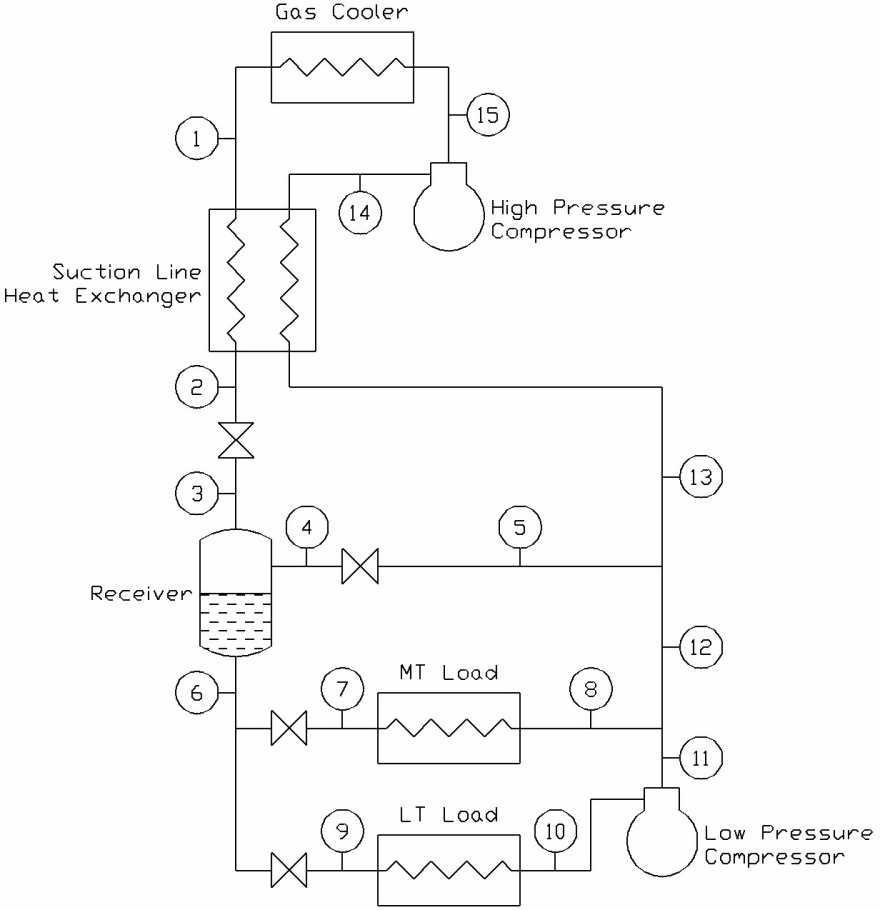
\includegraphics[width=0.9\textwidth, height=0.9\textheight, keepaspectratio=true]{media/image6337.png}
\caption{Schematic of the Transcritical CO\$\_\{2\}\$ Booster Refrigeration Cycle. \protect \label{fig:schematic-of-the-transcritical-co_2-booster}}
\end{figure}

\begin{figure}[hbtp] % fig 290
\centering
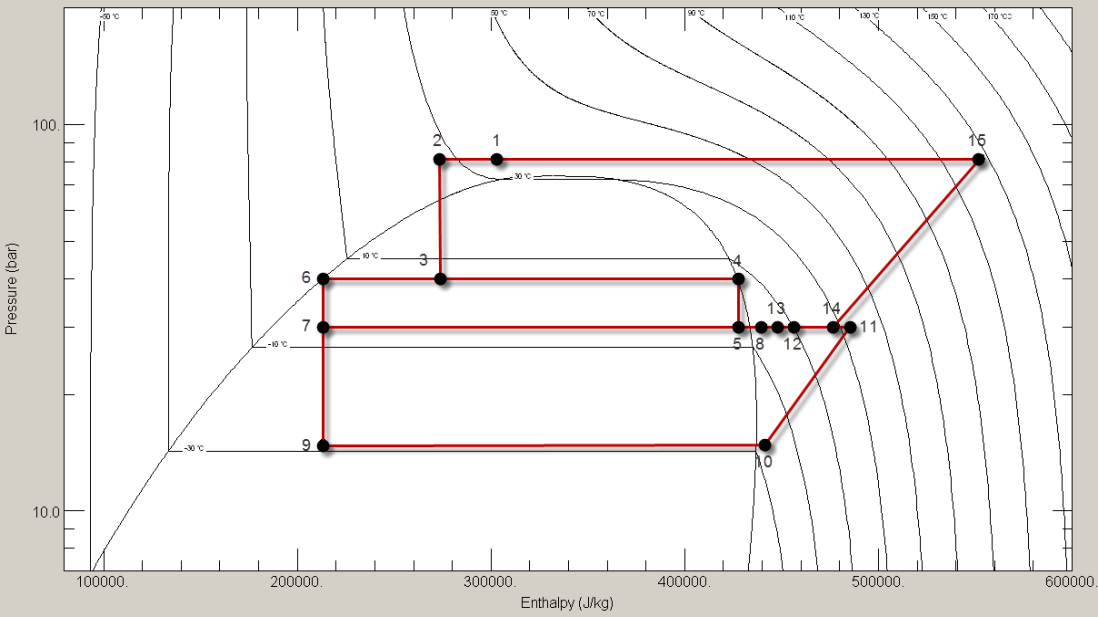
\includegraphics[width=0.9\textwidth, height=0.9\textheight, keepaspectratio=true]{media/image6338.png}
\caption{Pressure-Enthalpy (*p-H*) Diagram for the Transcritical CO\$\_\{2\}\$ Booster Refrigeration Cycle. \protect \label{fig:pressure-enthalpy-p-h-diagram-for}}
\end{figure}

Carbon dioxide exits the gas cooler at Location~1 and passes through the suction line heat exchanger, exiting at Location~2, during which the refrigerant is cooled by the suction gas.~ An intermediate expansion occurs between Locations~2 and~3, and saturated CO\(_{2}\) enters the receiver.~ Saturated liquid CO\(_{2}\) exits the receiver at Location~6, which is then expanded and fed to the medium-temperature loads (between Locations~7 and~8) and the low-temperature loads (between Locations~9 and~10).~ Saturated vapor CO\(_{2}\) exits the receiver bypass at Location~4 and is expanded to the medium-temperature pressure level at Location~5.~ Carbon dioxide vapor exiting the low temperature loads is compressed to the medium-temperature pressure level (Location~10 to 11).~ The CO\(_{2}\) from the discharge of the low pressure compressors, the outlet of the medium-temperature loads and the outlet of the receiver bypass are then combined at Location~13.~ The CO\(_{2}\) suction gas then passes through the suction line heat exchanger where the refrigerant is heated, exiting at Location~14.~ The carbon dioxide is finally compressed to the gas cooler pressure level at Location~15 and heat is rejected to the surroundings in the gas cooler between Locations~15 and~1.

\subsubsection{CO\(_{2}\) Compressor Performance Modeling}\label{coux5f2-compressor-performance-modeling}

To model the performance of the CO\(_{2}\) compressors during subcritical and transcritical operation, cubic polynomials are used to curve fit manufacturers' performance data.~ This technique is similar to that described in AHRI Standard 540 (AHRI 2004).~ For subcritical operation, the power consumption and cooling capacity of a CO\(_{2}\) compressor is a function of the saturated suction temperature, \emph{t\(_{ss}\)} (\(^{\circ}\)C), and the saturated discharge temperature, \emph{t\(_{sd}\)} (\(^{\circ}\)C), as follows:

\begin{equation}
z = {C_1} + {C_2}{t_{ss}} + {C_3}{t_{sd}} + {C_4}t_{ss}^2 + {C_5}{t_{ss}}{t_{sd}} + {C_6}t_{sd}^2 + {C_7}t_{ss}^3 + {C_8}t_{ss}^2{t_{sd}} + {C_9}{t_{ss}}t_{sd}^2 + {C_{10}}t_{sd}^3
\end{equation}

where \emph{z} is either power consumption (W) or cooling capacity (W) and \emph{C\(_{x}\)} are the corresponding correlation coefficients.

For transcritical operation, the power consumption (in Watts) of a CO\(_{2}\) compressor, \emph{W}, is a function of the saturated suction temperature and the gas cooler pressure, \emph{p\(_{gc}\)} (Pa), as follows (Ge and Tassou 2011):

\begin{equation}
W = {C_1} + {C_2}{t_{ss}} + {C_3}{p_{gc}} + {C_4}t_{ss}^2 + {C_5}{t_{ss}}{p_{gc}} + {C_6}p_{gc}^2 + {C_7}t_{ss}^3 + {C_8}t_{ss}^2{p_{gc}} + {C_9}{t_{ss}}p_{gc}^2 + {C_{10}}p_{gc}^3
\end{equation}

The cooling capacity (in Watts) of a transcritical CO\(_{2}\) compressor, \emph{Q}, is a function of the saturated suction temperature and the gas cooler outlet enthalpy, \emph{h\(_{go}\)} (J/kg), as follows (Ge and Tassou 2011):

\begin{equation}
Q = {C_1} + {C_2}{t_{ss}} + {C_3}{h_{go}} + {C_4}t_{ss}^2 + {C_5}{t_{ss}}{h_{go}} + {C_6}h_{go}^2 + {C_7}t_{ss}^3 + {C_8}t_{ss}^2{h_{go}} + {C_9}{t_{ss}}h_{go}^2 + {C_{10}}h_{go}^3
\end{equation}

The correlation coefficients, \emph{C\(_{x}\)}, are obtained either directly from CO\(_{2}\) compressor manufacturers or from cubic curve fits performed on their published CO\(_{2}\) compressor performance data.~ For convenience, correlation coefficients for CO\(_{2}\) compressors from several manufacturers have been included in the EnergyPlus refrigeration compressor coefficient database.

The rated values for the cooling capacity and power consumption from the manufacturer include a specified amount of subcooling before the thermal expansion valve and a certain amount of superheat in the suction gas.~ Adjustments must be made to these rated values to reflect the actual subcooling and superheat conditions.~ Actual subcooling is determined by the condenser's rated subcooling and by the subcooling provided by optional subcoolers. The actual superheat is determined by the refrigerated case superheat (usually set to ensure that there is no liquid in the suction lines leading to the compressors), set here at 10\(^{\circ}\)C, and the effect from any optional subcoolers.~ See the section, ``Detailed Refrigeration Systems'', for a description of the compressor corrections.

Once the corrected capacity is calculated for each compressor, the compressors are dispatched one at a time until the system load is met.~ The last compressor dispatched is assumed to run at full load for the fraction of the time step necessary to meet the load.~ That is, the model neglects compressor cycling losses at part-load conditions.~ If the capacity available from all the compressors is less than the sum of the case loads for that time period, the unmet load is accumulated to be met in succeeding time steps.~ If this accumulated unmet load becomes too great, a warning message is generated.

\subsubsection{Gas Cooler Performance}\label{gas-cooler-performance}

Only one gas cooler is allowed per transcritical refrigeration system. However, multiple refrigeration systems can reject heat through the same gas cooler.~ Currently, only air-cooled gas coolers are modeled.~ The gas cooler performance is modeled to determine the gas cooler pressure, gas cooler outlet temperature and outlet enthalpy of the refrigerant, and the auxiliary power consumption for the fans.

\paragraph{Optimal Gas Cooler Pressure for Transcritical CO\(_{2}\) Cycles}\label{optimal-gas-cooler-pressure-for-transcritical-coux5f2-cycles}

When the compressor discharge conditions are such that the CO\(_{2}\) is in the supercritical region, then the high-side operating pressure is independent of the gas cooler exit temperature (Sawalha 2008).~ Thus, for a given gas cooler exit temperature, there is an optimum pressure to achieve the maximum coefficient of performance (COP).~ Figure~\ref{fig:cop-of-co_2-transcritical-cycle-vs.-discharge} illustrates the variation in COP of a transcritical CO\(_{2}\) cycle with discharge pressure at different gas cooler exit temperatures.

\begin{figure}[hbtp] % fig 291
\centering
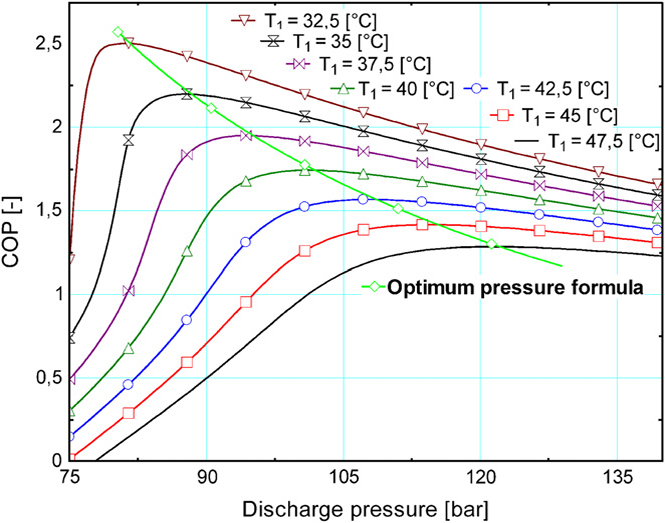
\includegraphics[width=0.9\textwidth, height=0.9\textheight, keepaspectratio=true]{media/image6342.png}
\caption{COP of CO\(_2\) Transcritical Cycle vs. Discharge Pressure at Different Gas Cooler Exit Temperatures (Sawalha 2008). \protect \label{fig:cop-of-co_2-transcritical-cycle-vs.-discharge}}
\end{figure}

Several researchers have developed correlations to determine the optimum gas cooler pressure in CO\(_{2}\) refrigeration systems (Chen and Gu 2005; Ge and Tassou 2011; Kauf 1998; Liao and Zhao 2000; Sawalha 2008).~ Using a similar curve-fitting procedure, the following optimum gas cooler pressure correlations are used in EnergyPlus:

\begin{equation}
  p_{gc} = \left\{
             \begin{array}{cl}
               7.5 \times 10^6                                & if~T_{amb} <    27^{\circ}C \\
               2.3083 \times 10^5 T_{amb} + 1.190 \times 10^6 & if~T_{amb} \geq 27^{\circ}C
             \end{array}
           \right.
\end{equation}

where \emph{p\(_{gc}\)} is the optimum gas cooler pressure (Pa) and \emph{T\(_{amb}\)} (\(^{\circ}\)C) is the ambient temperature surrounding the gas cooler.~ The corresponding gas cooler exit temperature, \emph{T\(_{gco}\)} (\(^{\circ}\)C), is determined as follows:

\begin{equation}
{T_{gco}} = {T_{amb}} + \Delta {T_{approach}}
\end{equation}

where \(\Delta T_{approach}\) is the approach temperature of the gas cooler, defined as the difference between the gas cooler exit temperature and the entering ambient air temperature.

During transcritical operation, the gas cooler outlet pressure is not allowed to fall below 7.5~×~10\(^{6}\)~Pa to ensure proper operation.

\paragraph{Condensing Temperature and Pressure for Subcritical Operation}\label{condensing-temperature-and-pressure-for-subcritical-operation}

During subcritical operation, the gas cooler behaves as a condenser and the condensing pressure is allowed to float with the ambient conditions.~ The condensing temperature, \emph{T\(_{cond}\)} (°C), is determined according to the following:

\begin{equation}
  T_{cond} = \left\{
               \begin{array}{cl}
                 T_{cond,min}                           & if~T_{amb} \le T_{cond,min} - \Delta T \\
                 T_{amb} + \Delta T                     & if~T_{cond,min} - \Delta T < T_{amb} \le T_{trans} - \Delta T \\
                 T_{trans}                              & if~T_{trans} - \Delta T < T_{amb} < T_{trans} \\
                 T_{sat,P = 7.2MPa}                     & if~T_{trans} \le {T_{amb}} < 30.978 
               \end{array}
             \right.
\end{equation}

where \(T_{amb}\) is the ambient temperature (\(^{\circ}\)C), \(\Delta T\) is the temperature difference between the condensing temperature and the ambient temperature (\(^{\circ}\)C), \(T_{cond,min}\) is the minimum allowable condensing temperature (\(^{\circ}\)C), and \(T_{trans}\) is the ambient air transition temperature between subcritical and transcritical operation (\(^{\circ}\)C).~ The condensing pressure, \(P_{cond}\) (Pa), is determined as the saturation pressure corresponding to the condensing temperature.

\paragraph{Gas Cooler Fan Energy Use}\label{gas-cooler-fan-energy-use}

Gas cooler fan power for air-cooled gas coolers is determined by the type of fan control, which can either be fixed, variable speed, or two-speed.~ For all three fan control types, the gas cooler fan energy is calculated in the same fashion as that for air-cooled condensers, as described in the section, ``Detailed Refrigeration Systems''.

\subsubsection{Suction Line Heat Exchanger}\label{suction-line-heat-exchanger}

The performance of the transcritical CO\(_{2}\) booster system can be enhanced by using a suction line heat exchanger.~ As shown in Figure~\ref{fig:schematic-of-the-transcritical-co_2-booster}, the suction gas entering the heat exchanger at location 13 is used to cool the refrigerant after it leaves the gas cooler at location 1.~ The performance of this heat exchanger is modeled with the heat exchanger effectiveness, \(\varepsilon\):

\begin{equation}
\varepsilon  = \frac{{{h_{14}} - {h_{13}}}}{{{h_{{T_1},{P_{13}}}} - {h_{13}}}} = \frac{{{h_1} - {h_2}}}{{{h_{{T_1},{P_{13}}}} - {h_{13}}}}
\end{equation}

where \emph{h}\(_{1}\), \emph{h}\(_{2}\), \emph{h}\(_{13}\), and \emph{h}\(_{14}\) are the enthalpies of carbon dioxide at the respective locations in the refrigeration cycle, as shown in Figure~\ref{fig:schematic-of-the-transcritical-co_2-booster} and Figure~\ref{fig:pressure-enthalpy-p-h-diagram-for}, and \({h_{{T_1},{P_{13}}}}\) ~is the enthalpy of carbon dioxide evaluated at temperature \emph{T}\(_{1}\) and pressure \emph{P}\(_{13}\).

In EnergyPlus, the value of the suction line heat exchanger effectiveness, \(\varepsilon\), is specified by the user as an input, and the enthalpies at the exit of the heat exchanger, \emph{h}\(_{2}\) and \emph{h}\(_{14}\), are determined from the definition of heat exchanger effectiveness given above.~ In EnergyPlus, the default value of heat exchanger effectiveness is 0.4.

\textbf{Thermodynamic Properties of CO\(_{2}\)}

Modeling of transcritical CO\(_{2}\) booster refrigeration cycles requires the thermodynamic properties of CO\(_{2}\) in the saturated (liquid and vapor), superheated and supercritical regions.~ The refrigerant properties database within EnergyPlus includes saturated, superheated and supercritical thermodynamic data for CO\(_{2}\), including temperature, pressure, density, enthalpy and specific heat.

\subsection{References}\label{references-040}

AHRI, 2001. Standard 410, Forced-Circulation Air-Cooling and Air-Heating Coils, Section 6.2.1, Air-Conditioning Heating \& Refrigeration Institute

ARI. 2003. Standard for Remote Mechanical-Draft Evaporatively-Cooled Refrigerant Condensers, Standard 490, Air-Conditioning \& Refrigeration Institute, Arlington, VA

ARI. 2004. Standard for Performance Rating of Positive Displacement Refrigerant Compressors and Compressor Units, Standard 540, Air-Conditioning \& Refrigeration Institute, Arlington, VA

ARI. 2005. Standard for Performance Rating of Remote Mechanical-Draft Air-Cooled Refrigerant Condensers, Standard 460, Air-Conditioning \& Refrigeration Institute, Arlington, VA

ARI. 2007. Standard for Performance Rating of Water-Cooled Refrigerant Condensers, Remote Type, Standard 450, Air-Conditioning \& Refrigeration Institute, Arlington, VA

ASHRAE. 2002. \emph{Refrigeration Handbook}, Chapter 47. Atlanta: American Society of Heating, Refrigerating and Air-Conditioning Engineers, Inc.

ASHRAE. 2004. \emph{HVAC Systems and Equipment Handbook}, Atlanta: American Society of Heating, Refrigerating and Air-Conditioning Engineers, Inc.

ASHRAE. 2006a. \emph{Refrigeration Handbook}, Chapter 2. Atlanta: American Society of Heating, Refrigerating and Air-Conditioning Engineers, Inc.

ASHRAE. 2006b. \emph{Refrigeration Handbook}, Chapter 44. Atlanta: American Society of Heating, Refrigerating and Air-Conditioning Engineers, Inc.

ASHRAE. 2006c. \emph{Refrigeration Handbook}, Chapter 4. Atlanta: American Society of Heating, Refrigerating and Air-Conditioning Engineers, Inc.

ASHRAE. 2006d. \emph{Refrigeration Handbook}, Chapter 13. Atlanta: American Society of Heating, Refrigerating and Air-Conditioning Engineers, Inc.

ASHRAE. 2009. \emph{Fundamentals Handbook}, Chapter 1. Atlanta: American Society of Heating, Refrigerating and Air-Conditioning Engineers, Inc.

ASHRAE. 2009b. \emph{Fundamentals Handbook}, Chapter 2. Atlanta: American Society of Heating, Refrigerating and Air-Conditioning Engineers, Inc.

B.A.C. 2007. Baltimore AirCoil Company Product and Application Handbook, Volume II, Baltimore, MD

Baek, J.S., Groll, E.A., and Lawless, P.B. 2005. Theoretical Performance of Transcritical Carbon Dioxide Cycle with Two-Stage Compression and Intercooling. \emph{Proceedings of the Institution of Mechanical Engineers, Part E: Journal of Process Mechanical Engineering} 219, 187-195.

Baxter, V. D., Mei, V.C. 2002.Warm Liquid Defrosting Technology For Supermarket Display Cases, P.S. Hrnjak, Ed., International Conference New Technologies in Commercial Refrigeration, University of Illinois at Urbana-Champaign, Urbana, IL, July 22-23, 2002

Chen, Y., and Gu, J. 2005. The Optimum High Pressure for CO\(_{2}\) Transcritical Refrigeration Systems with Internal Heat Exchangers. \emph{International Journal of Refrigeration} 28(8), 1238-1249.

Evans, J. 2008. Chapter 15, Minimising Energy Consumption Associated with Chilling, Refrigerated Storage and Cooling Systems in the Food Industry. In \emph{Handbook of Water and Energy Management in Food Processing}. Cambridge:~ Woodhead Publishing Limited.

Faramarzi, R. T., and Walker, D. H. 2004. Investigation of Secondary Lop Supermarket Refrigeration Systems, prepared for California Energy Commission Public Interest Energy Research Program, prepared by Southern California Edison and Foster-Miller, PIER 500-04-013

Ge, Y., and Tassou, S. 2011. Performance Evaluation and Optimal Design of Supermarket Refrigeration Systems with Supermarket Model ``Supersim'', Part I: Model Description and Validation. \emph{International Journal of Refrigeration} 34(2), 527-539.

Gosney, W.B., Olama, G.A.-L. 1975. Heat and Enthalpy Gains through Cold Room Doorways,~ Proceedings of the Institute of Refrigeration, vol.~72, pp 31-41

Henderson, H.I. and Khattar, M. 1999. Measured Impacts of Supermarket Humidity Level on Defrost Performance and Refrigerating System Energy Use. \emph{ASHRAE Transactions} 105(1), 508-520. Atlanta: American Society of Heating, Refrigerating and Air-Conditioning Engineers, Inc.

Hinde, D., Zha, S., and Lan, L. 2009. Carbon Dioxide in North American Supermarkets, ASHRAE Journal, Atlanta: American Society of Heating, Refrigerating and Air-Conditioning Engineers, Inc.,February 2009

Howell, R.H. 1993. Effects of Store Relative Humidity on Refrigerated Display Case Performance. \emph{ASHRAE Transactions} 99(1), 667-678. Atlanta: American Society of Heating, Refrigerating and Air-Conditioning Engineers, Inc.

Howell, R.H. 1993. Calculation of Humidity Effects on Energy Requirements of Refrigerated Display Cases. \emph{ASHRAE Transactions} 99(1), 679-693. Atlanta: American Society of Heating, Refrigerating and Air-Conditioning Engineers, Inc.

IEA Heat Pump Centre. 2003. \emph{Advanced Supermarket Refrigeration/Heat Recovery Systems Vol. 1 - Executive Summary}, Report HPP-AN26-2, April.

ITT. 2009. Goulds Pumps Industrial~ Products Moter Terms

Kauf, F. 1998. Determination of the Optimum High Pressure for Transcritical CO\(_{2}\)-Refrigeration Cycles. \emph{International Journal of Thermal Sciences} 38(4), 325-330.

Kays, W.M., A.L. London, 1964, compact Heat Exchangers, Second Edition, Chap. 2, pp 15-24, McGraw-Hill Book Company

Kazachki, G. S., and Hinde, D. K. 2006, Secondary Cooplant Systems for Supermarkets, ASHRAE Journal, Atlanta: American Society of Heating, Refrigerating and Air-Conditioning Engineers, Inc., September 2006

Lawrence Berkeley Laboratory and Resource Dynamics, Improving Fan System Performance, A Sourcebook for Industry, DOE/GO-102003-1294, April 2003

Lee, T-S., Liu, C-H., and Chen, T-W. 2006. Thermodynamic Analysis of Optimal Condensing Temperature of Cascade-Condenser in CO\(_{2}\)/NH\(_{3}\) Cascade Refrigeration Systems, International Journal of Refrigeration 29 (2006) 1100-1108, Elsevier Ltd.

Liao, S., and Zhao, T. J. 2000. A Correlation of Optimal Heat Rejection Pressures in Transcritical Carbon Dioxide Cycles. \emph{Applied Thermal Engineering} 20(9), 831-841.

Manske, K.A., 2000. Performance Optimization of Industrial Refrigeration Systems, M.S.Thesis Mechanical Engineering, Solar Energy Laboratory, University of Wisconsin-Madison.

Minea, V. 2007. Supermarket Refrigeration System with Completely Secondary Loops, ASHRAE Journal, Atlanta: American Society of Heating, Refrigerating and Air-Conditioning Engineers, Inc., ~September 2007

Mitchell, J.W., et al. 1992.Analysis of Supermarket Dehumidification Alternatives. Final Report to Electric Power Research Institute, Report TR-100352, November.

NASA. 1976. U. S. Standard Atmosphere, NASA-TM-74335, National Oceanic and Atmospheric Administration , National Aeronautics and Space Administration

Nelson, B. I., 2010, Refrigeration Air Cooler Rating Methods, ASHRAE Journal, American Society of Heating, Refrigeration and Air-Conditioning Engineers, Inc., August

Sawalha, S. 2008. Theoretical Evaluation of Trans-Critical CO\(_{2}\) Systems in Supermarket Refrigeration. Part I: Modeling, Simulation and Optimization of Two System Solutions. \emph{International Journal of Refrigeration} 31, 516-524.

Terrell, W.J.Jr., Mao, Y., Hrnjak, P.S. 1999. Evaluation of Secondary Fluids for Use in Low-Temperature Supermarket Applications, ACRC CR-15, Air Conditioning and Refrigeration Center, University of Illinois, Urbana, IL, April 1999.
